% =================================================================
%  Elevator Vertical Distance Estimation -- Research Presentation
%  Authors: Eyal Yakir, Uriya Cohen-Eliya
%  Theme:  Metropolis (customised, copper-accent)
%  Build:  pdflatex presentation.tex   (run twice for TOC)
% =================================================================
\documentclass[aspectratio=169,11pt]{beamer}

\usetheme[progressbar=frametitle, sectionpage=progressbar, numbering=fraction, block=fill]{metropolis}
\usepackage{appendixnumberbeamer}
\usepackage[T1]{fontenc}
\usepackage[utf8]{inputenc}
\usepackage{textcomp}
\usepackage{lmodern}
\usepackage{amsmath, amssymb}
\usepackage{xcolor}
\usepackage{graphicx}
\usepackage{tikz}
\usetikzlibrary{positioning, arrows.meta, calc, fit, backgrounds}
\usepackage{booktabs}
\usepackage{array}
\usepackage{tabularx}

% -----------------------------------------------------------------
%  COLOURS
% -----------------------------------------------------------------
\definecolor{pgbg}{HTML}{FAF7F2}
\definecolor{pgtext}{HTML}{1B2A47}
\definecolor{pgcopper}{HTML}{B5651D}
\definecolor{pgsage}{HTML}{5A7A5A}
\definecolor{pgred}{HTML}{A0382F}
\definecolor{pgsteel}{HTML}{3E5C76}
\definecolor{pgcard}{HTML}{F1ECE2}
\definecolor{pglight}{HTML}{C9C2B6}
\definecolor{pggrey}{HTML}{4A4A4A}

% -----------------------------------------------------------------
%  THEME OVER-RIDES
% -----------------------------------------------------------------
\setbeamercolor{normal text}{fg=pgtext, bg=pgbg}
\setbeamercolor{alerted text}{fg=pgcopper}
\setbeamercolor{example text}{fg=pgsage}

\setbeamercolor{frametitle}{fg=pgbg, bg=pgtext}
\setbeamercolor{progress bar}{fg=pgcopper}
\setbeamercolor{title separator}{fg=pgcopper}
\setbeamercolor{progress bar in head/foot}{fg=pgcopper}
\setbeamercolor{progress bar in section page}{fg=pgcopper}

\setbeamercolor{block title}{fg=pgcopper, bg=pgcard}
\setbeamercolor{block body}{fg=pgtext, bg=pgcard}

\setbeamercolor{section in toc}{fg=pgtext}
\setbeamercolor{footnote}{fg=pggrey}
\setbeamercolor{caption name}{fg=pgcopper}
\setbeamercolor{caption}{fg=pggrey}

\setbeamerfont{title}{series=\bfseries, size=\Huge}
\setbeamerfont{subtitle}{shape=\itshape, size=\large}
\setbeamerfont{frametitle}{series=\bfseries, size=\Large}
\setbeamerfont{caption}{shape=\itshape, size=\footnotesize}

\setbeamertemplate{itemize item}{\textcolor{pgcopper}{\rule[0.5ex]{1ex}{1ex}}}
\setbeamertemplate{itemize subitem}{\textcolor{pgsteel}{\textbullet}}

% -----------------------------------------------------------------
%  HELPERS — fixed-height cards for consistency
% -----------------------------------------------------------------
% \fcard{accent}{width}{height}{content}  — fixed-height card with top stripe
\newcommand{\fcard}[4]{%
  \begin{tikzpicture}
    \node[rectangle, fill=pgcard, draw=none, inner sep=0pt,
          minimum width=#2, minimum height=#3, anchor=north west] (cb) at (0,0) {};
    \node[anchor=north west, inner sep=10pt,
          text width=\dimexpr#2-20pt, text=pgtext] at ([yshift=-3pt]cb.north west)
          {\begin{minipage}[t][\dimexpr#3-13pt][t]{\dimexpr#2-20pt}#4\end{minipage}};
    \fill[#1] (cb.north west) rectangle ([xshift=#2, yshift=-3pt]cb.north west);
  \end{tikzpicture}%
}

% Big stat card: \stat{accent}{width}{value}{label}
\newcommand{\stat}[4]{%
  \begin{tikzpicture}
    \node[rectangle, fill=pgcard, minimum width=#2, minimum height=2.4cm,
          anchor=north west, inner sep=0pt] (s) at (0,0) {};
    \node[anchor=north west, inner sep=12pt] at ([yshift=-3pt]s.north west)
      {\begin{minipage}[t][2.0cm][t]{\dimexpr#2-24pt}
        {\color{#1}\fontsize{30pt}{34pt}\selectfont\bfseries #3}\\[0.15cm]
        {\color{pgtext}\itshape\small #4}
       \end{minipage}};
    \fill[#1] (s.north west) rectangle ([xshift=#2, yshift=-3pt]s.north west);
  \end{tikzpicture}%
}

% Small stat (for Phones / Labelled rides etc)
\newcommand{\smallstat}[3]{%
  \begin{tikzpicture}
    \node[rectangle, fill=pgcard, minimum width=#1, minimum height=1.5cm,
          anchor=north west, inner sep=0pt] (s) at (0,0) {};
    \node[anchor=north, inner sep=0pt] at ([yshift=-0.20cm]s.north)
      {\color{pgcopper}\fontsize{22pt}{24pt}\selectfont\bfseries #2};
    \node[anchor=south, inner sep=0pt] at ([yshift=0.18cm]s.south)
      {\color{pgtext}\itshape\footnotesize #3};
    \fill[pgcopper] (s.north west) rectangle ([xshift=#1, yshift=-3pt]s.north west);
  \end{tikzpicture}%
}

% Agenda item: \agenda{accent}{width}{number}{title}{body}
\newcommand{\agenda}[5]{%
  \begin{tikzpicture}
    \node[rectangle, fill=pgcard, minimum width=#2, minimum height=1.45cm,
          anchor=north west, inner sep=0pt] (a) at (0,0) {};
    \node[anchor=west, inner sep=0pt] at ([xshift=10pt]a.west)
      {\color{#1}\Large\bfseries #3};
    \node[anchor=north west, inner sep=0pt] at ([xshift=58pt, yshift=-12pt]a.north west)
      {\color{pgtext}\bfseries #4};
    \node[anchor=north west, inner sep=0pt, text=pggrey] at ([xshift=58pt, yshift=-32pt]a.north west)
      {\begin{minipage}[t]{\dimexpr#2-70pt}\footnotesize #5\end{minipage}};
    \fill[#1] (a.north west) rectangle ([xshift=4pt, yshift=-1.45cm]a.north west);
  \end{tikzpicture}%
}

% -----------------------------------------------------------------
%  TITLE METADATA
% -----------------------------------------------------------------
\title{Elevator Vertical Distance Estimation}
\subtitle{Predicting how far an elevator travelled\\using only the sensors in your pocket.}
\author{Eyal Yakir \and Uriya Cohen-Eliya}
\institute{Smartphone Inertial \& Pressure Sensing}
\date{April 2026}

% Custom title page
\setbeamertemplate{title page}{%
\begin{tikzpicture}[remember picture, overlay]
  \draw[pgcopper, line width=1.4pt]
        ([yshift=-0.55cm]current page.north west) --
        ([yshift=-0.55cm]current page.north east);
  \node[anchor=north west, text=pgcopper, font=\bfseries\small]
        at ([xshift=0.8cm,yshift=-0.85cm]current page.north west)
        {RESEARCH REPORT \, \textperiodcentered \, 2026};
  \node[anchor=west, text=pgtext, align=left,
        font=\fontsize{34pt}{40pt}\selectfont\bfseries]
        at ([xshift=0.9cm, yshift=0.4cm]current page.west)
        {Elevator Vertical\\Distance Estimation};
  \node[anchor=north west, text=pgsteel, font=\large\itshape, text width=12cm]
        at ([xshift=0.9cm, yshift=-1.6cm]current page.center)
        {Predicting how far an elevator travelled\\using only the sensors in your pocket.};
  \draw[pgcopper, line width=1.6pt]
        ([xshift=0.9cm,  yshift=-2.7cm]current page.center) --
        ([xshift=4.0cm,  yshift=-2.7cm]current page.center);
  \node[anchor=north west, text=pgtext, font=\bfseries\large]
        at ([xshift=0.9cm,  yshift=-3.0cm]current page.center)
        {Eyal Yakir \, \textperiodcentered \, Uriya Cohen-Eliya};
  \node[anchor=north west, text=pggrey, font=\small]
        at ([xshift=0.9cm,  yshift=-3.55cm]current page.center)
        {Smartphone Inertial \& Pressure Sensing};
\end{tikzpicture}}

% Custom section page
\setbeamertemplate{section page}{%
\begin{tikzpicture}[remember picture, overlay]
  \node[anchor=center, text=pgtext, font=\fontsize{36pt}{42pt}\selectfont\bfseries]
        at (current page.center) {\insertsectionhead};
  \draw[pgcopper, line width=2pt]
        ([yshift=-0.8cm]current page.center) ++(-1.5cm,0) --
        ([yshift=-0.8cm]current page.center) ++(1.5cm,0);
\end{tikzpicture}}

% -----------------------------------------------------------------
\begin{document}

% =================================================================
%  TITLE PAGE
% =================================================================
{\setbeamertemplate{footline}{}
\begin{frame}[plain,noframenumbering]
  \titlepage
\end{frame}}


% =================================================================
%  ACT I -- INTRODUCTION
% =================================================================

% ---------- The Problem ----------
\begin{frame}{The Problem}
\centering
{\itshape\large\color{pgsteel}
A phone in your pocket. An elevator ride.\\
How far did you actually travel\, --\, vertically?}\par
\vspace{0.6cm}
\begin{columns}[T,onlytextwidth]
\column{0.32\linewidth}
\fcard{pgcopper}{\linewidth}{4.5cm}{%
{\color{pgcopper}\Huge\bfseries a}\\[6pt]
{\color{pgtext}\bfseries Detect\\the ride}\\[6pt]
{\color{pggrey}\small Find when the elevator started and stopped\, --\, purely from the IMU.}}
\column{0.32\linewidth}
\fcard{pgsage}{\linewidth}{4.5cm}{%
{\color{pgsage}\Huge\bfseries b}\\[6pt]
{\color{pgtext}\bfseries Estimate\\$\Delta h$}\\[6pt]
{\color{pggrey}\small Predict the signed vertical distance (up or down) in metres.}}
\column{0.32\linewidth}
\fcard{pgred}{\linewidth}{4.5cm}{%
{\color{pgred}\Huge\bfseries c}\\[6pt]
{\color{pgtext}\bfseries Quantify\\uncertainty}\\[6pt]
{\color{pggrey}\small Return a calibrated 90\,\% confidence interval\, --\, not just a point estimate.}}
\end{columns}
\end{frame}


% ---------- End-to-End Pipeline ----------
\begin{frame}{End-to-End Pipeline}
\textit{Two stages, one shared idea: model the physics, then quantify the noise.}\par
\vspace{0.7cm}
\centering
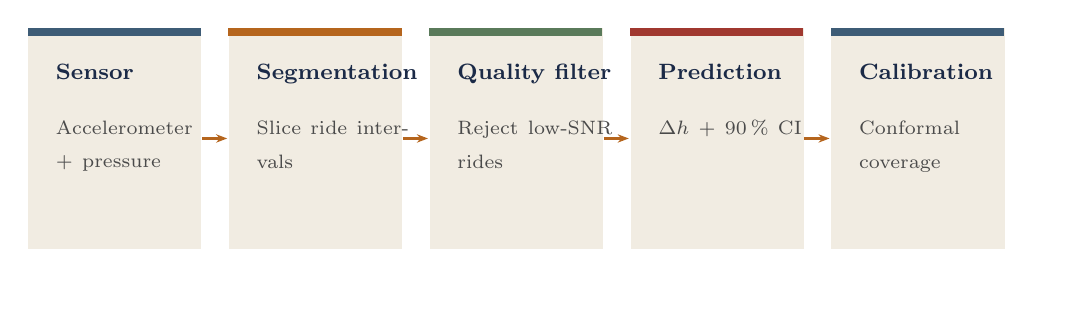
\begin{tikzpicture}[
  pipebox/.style={rectangle, fill=pgcard, draw=none,
                  minimum width=2.2cm, minimum height=2.8cm,
                  anchor=north west, inner sep=0pt},
  arrowstyle/.style={-{Stealth[length=4pt]}, color=pgcopper, line width=1.2pt}
]
\foreach \i/\c/\h/\b [count=\j from 0] in {%
  1/pgsteel/{Sensor}/{Accelerometer + pressure},%
  2/pgcopper/{Segmentation}/{Slice ride intervals},%
  3/pgsage/{Quality filter}/{Reject low-SNR rides},%
  4/pgred/{Prediction}/{$\Delta h$ + 90\,\% CI},%
  5/pgsteel/{Calibration}/{Conformal coverage}%
} {
  \pgfmathsetmacro{\xx}{\j*2.55}
  \node[pipebox] (n\i) at (\xx,0) {};
  \node[anchor=north west, inner sep=10pt,
        text width=2.0cm, text=pgtext] at ([yshift=-3pt]n\i.north west)
    {\begin{minipage}[t][2.6cm][t]{2.0cm}
       {\bfseries\footnotesize \h}\\[8pt]
       {\color{pggrey}\scriptsize \b}
     \end{minipage}};
  \fill[\c] (n\i.north west) rectangle ([xshift=2.2cm, yshift=-3pt]n\i.north west);
}
\foreach \a/\b in {1/2,2/3,3/4,4/5} {
  \draw[arrowstyle] (n\a.east) -- ([xshift=0.32cm]n\a.east);
}
\end{tikzpicture}
\par
\vspace{0.7cm}
{\color{pgcopper}\bfseries\small OUTPUT}\quad
{\color{pgtext}Per-ride signed $\Delta h$ in metres with calibrated $[\Delta\hat{h} - \delta,\, \Delta\hat{h} + \delta]$ interval.}
\end{frame}


% ---------- Data Collection ----------
\begin{frame}{Data Collection}
\textit{Multi-phone simultaneous recording across seven elevators in three cities.}\par
\vspace{0.4cm}
\centering
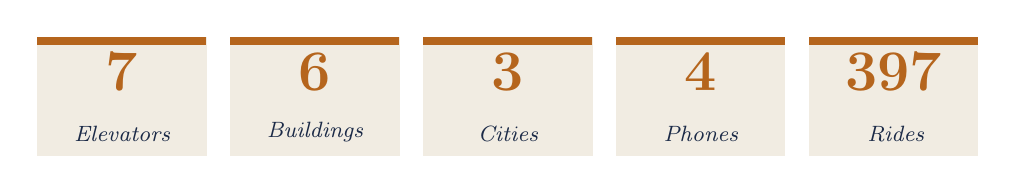
\begin{tikzpicture}
\foreach \i/\v/\l in {0/7/Elevators, 1/6/Buildings, 2/3/Cities, 3/4/Phones, 4/397/{\,Rides}} {
  \pgfmathsetmacro{\xx}{\i*2.45}
  \node[anchor=north west] (s\i) at (\xx,0) {\smallstat{2.15cm}{\v}{\l}};
}
\end{tikzpicture}
\par
\vspace{0.5cm}
\begin{columns}[T,onlytextwidth]
\column{0.50\linewidth}
{\color{pgcopper}\bfseries Buildings}\\
{\color{pgcopper}\rule{1.0cm}{0.8pt}}\\[2pt]
\scriptsize
\renewcommand{\arraystretch}{1.0}
\begin{tabular}{@{}p{4.4cm}p{2.6cm}@{}}
\textbf{Millenium\, --\, Internal}      & \textit{Ra'anana} \\
\textbf{Millenium\, --\, Outside}       & \textit{Ra'anana} \\
\textbf{Acro}                            & \textit{Ra'anana} \\
\textbf{Beit Mansour}                    & \textit{Ra'anana} \\
\textbf{Beit Yitzchaki}                  & \textit{held-out} \\
\textbf{BarIlan-2}                       & \textit{Herzliya} \\
\textbf{Haari}                           & \textit{Ramat Gan} \\
\end{tabular}
\column{0.50\linewidth}
{\color{pgcopper}\bfseries Protocol}\\
{\color{pgcopper}\rule{1.0cm}{0.8pt}}\\[2pt]
\scriptsize
\begin{itemize}\setlength\itemsep{0.5pt}
  \item Four phones recording in sync.
  \item Pattern: full traversal up, then descent.
  \item Stationary windows pre/post for gravity calibration.
  \item Barometer supplies GT where available.
\end{itemize}
\end{columns}
\end{frame}


% ---------- Storyline ----------
\begin{frame}{Storyline}
\textit{Where this hour will take us.}\par
\vspace{0.3cm}
\centering
\begin{columns}[T,onlytextwidth]
\column{0.48\linewidth}
\agenda{pgcopper}{\linewidth}{01}{Physics}{Jerk-limited S-curves and what an elevator looks like to an IMU.}
\par\vspace{4pt}
\agenda{pgsage}{\linewidth}{03}{Prediction}{Three algorithms: barometer, ZUPT, trapezoid pulse-pair.}
\par\vspace{4pt}
\agenda{pgcopper}{\linewidth}{05}{Results}{Held-out 89.4\% within $\pm$1.5\,m.}
\column{0.48\linewidth}
\agenda{pgsteel}{\linewidth}{02}{Detection}{Matched-filter pair detection on the accelerometer; F1 \& IoU.}
\par\vspace{4pt}
\agenda{pgred}{\linewidth}{04}{Uncertainty}{Per-segment $\sigma$, quality filter, conformal calibration.}
\par\vspace{4pt}
\agenda{pgsteel}{\linewidth}{06}{Product}{Streamlit Boutique Pipeline producing a Hebrew PDF.}
\end{columns}
\end{frame}


% ---------- Buildings chart ----------
\begin{frame}{Building Heights\, --\, Diversity of the Dataset}
\centering
\textit{Total traversable height per elevator. Spans short residential to multi-storey hotel.}\par
\vspace{0.2cm}
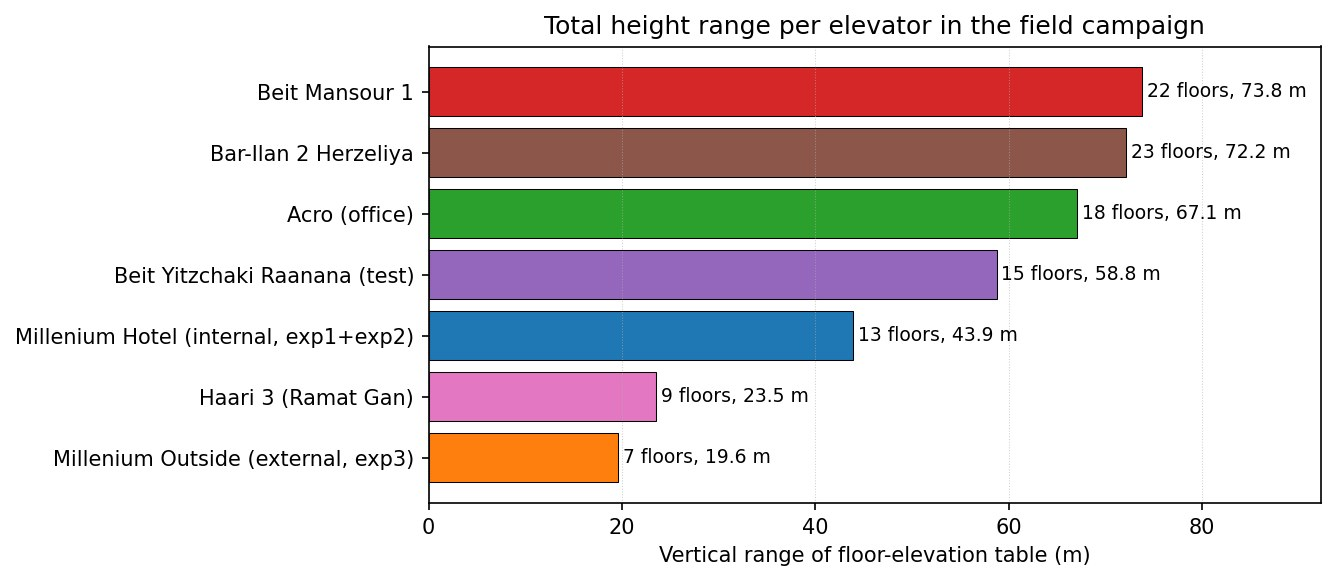
\includegraphics[width=0.82\linewidth, keepaspectratio]{presentation_figs/p003_i0.jpg}\par
\vspace{0.05cm}
{\footnotesize\itshape\color{pggrey}
Sum of signed $\Delta h$ across all rides per elevator.}
\end{frame}


% =================================================================
%  ACT II -- PHYSICS
% =================================================================
\section{Physics}

\begin{frame}{Elevator Kinematics: A Jerk-Limited S-Curve}
\begin{columns}[T,onlytextwidth]
\column{0.55\linewidth}
\centering
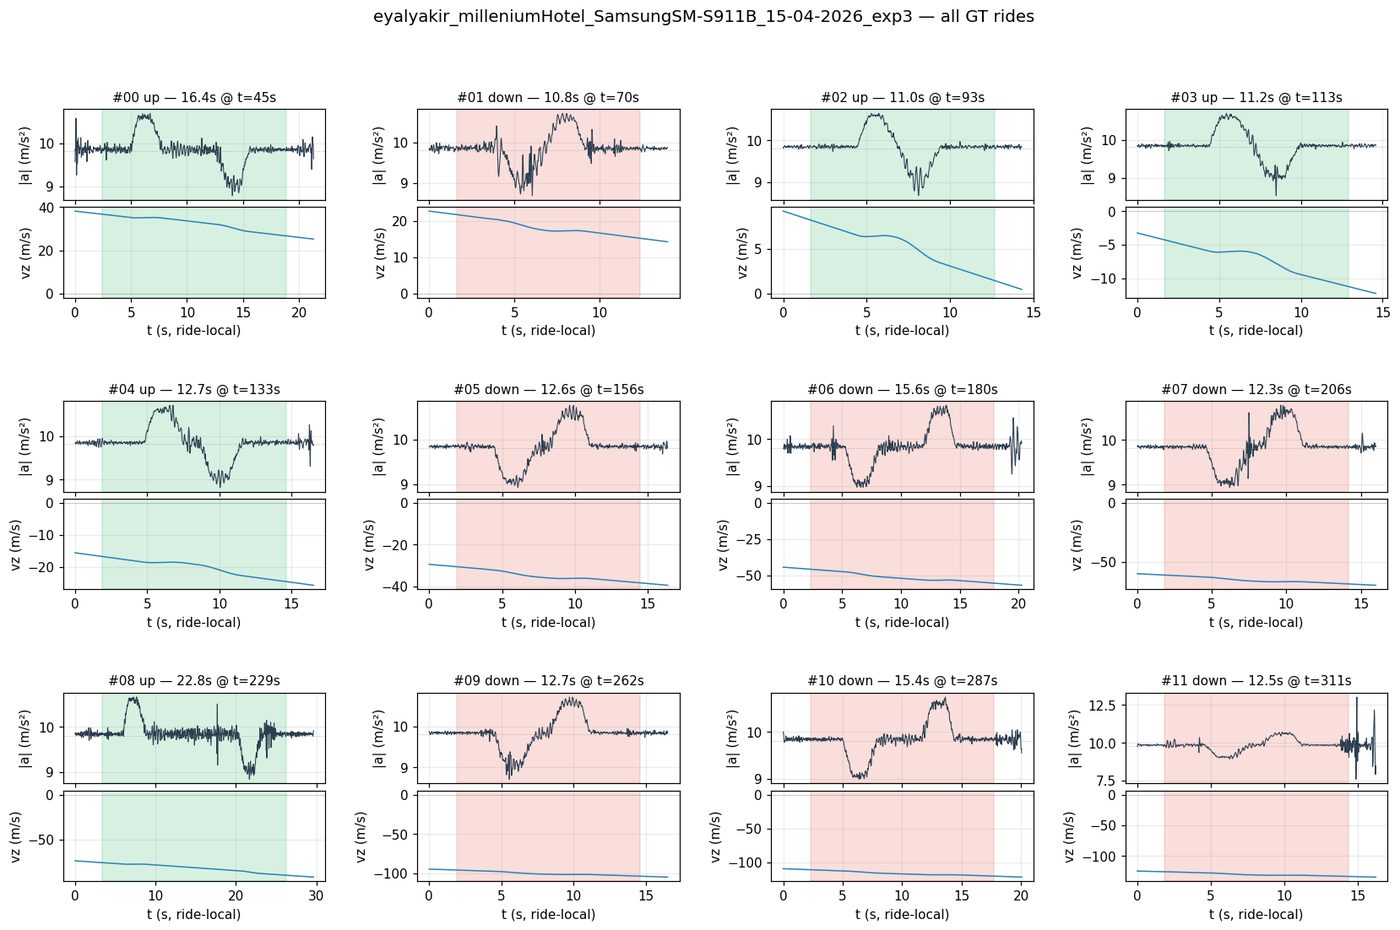
\includegraphics[width=\linewidth, keepaspectratio]{presentation_figs/p013_i0.jpg}
\column{0.43\linewidth}
{\color{pgcopper}\bfseries\large What the IMU sees}\\
{\color{pgcopper}\rule{1.4cm}{0.8pt}}\\[6pt]
\footnotesize
\textbf{Velocity $v(t)$}\\
Smooth S-curve\, --\, no kink at peak.\\[4pt]
\textbf{Acceleration $a(t)$}\\
Two trapezoid lobes\, --\, one positive, one negative.\\[4pt]
\textbf{Jerk}  $j(t) = \dddot{x}$\\
Bounded; this is what makes the ride comfortable.\\[4pt]
\textbf{Gravity dominates}\\
$|a| \ll g$.  Subtract carefully or estimates blow up.
\end{columns}
\end{frame}


\begin{frame}{Seven Phases of an Ideal Ride}
\centering
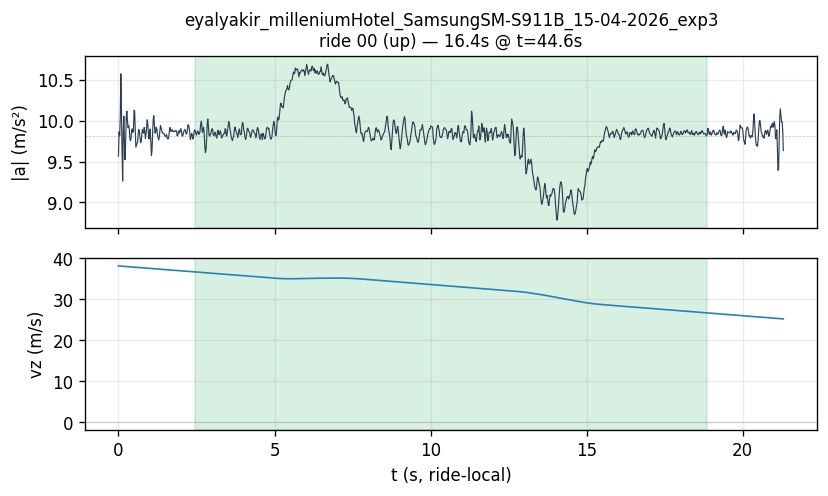
\includegraphics[width=0.82\linewidth, keepaspectratio]{presentation_figs/p012_i0.jpg}\par
\vspace{0.05cm}
{\footnotesize\itshape\color{pggrey}
Velocity (top) and acceleration (bottom) vs time. Seven phases mirror the jerk profile.}
\end{frame}


\begin{frame}{The Trapezoid Template: What We Actually Fit}
\begin{columns}[T,onlytextwidth]
\column{0.55\linewidth}
\centering
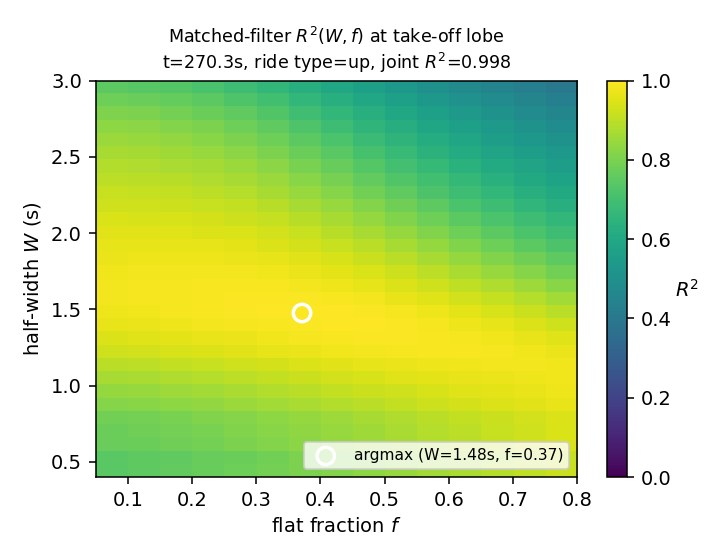
\includegraphics[width=\linewidth, keepaspectratio]{presentation_figs/p017_i0.jpg}
\column{0.43\linewidth}
{\color{pgcopper}\bfseries\large Why a trapezoid?}\\
{\color{pgcopper}\rule{1.4cm}{0.8pt}}\\[6pt]
\footnotesize
A perfect ride produces an acceleration profile composed of two trapezoid lobes:
positive at start, negative at end.\\[4pt]
We replace the smooth S-curve with this idealised shape.
Three free parameters per lobe:\\[10pt]

{\color{pgcopper}\Large\bfseries $a_0$} \quad {\color{pggrey}\itshape plateau amplitude}\\[8pt]
{\color{pgcopper}\Large\bfseries $\tau_r$} \quad {\color{pggrey}\itshape ramp duration}\\[8pt]
{\color{pgcopper}\Large\bfseries $\tau_p$} \quad {\color{pggrey}\itshape plateau duration}
\end{columns}
\end{frame}


% =================================================================
%  ACT III -- DETECTION
% =================================================================
\section{Detection}

\begin{frame}{Matched-Filter Detection}
\begin{columns}[T,onlytextwidth]
\column{0.55\linewidth}
\centering
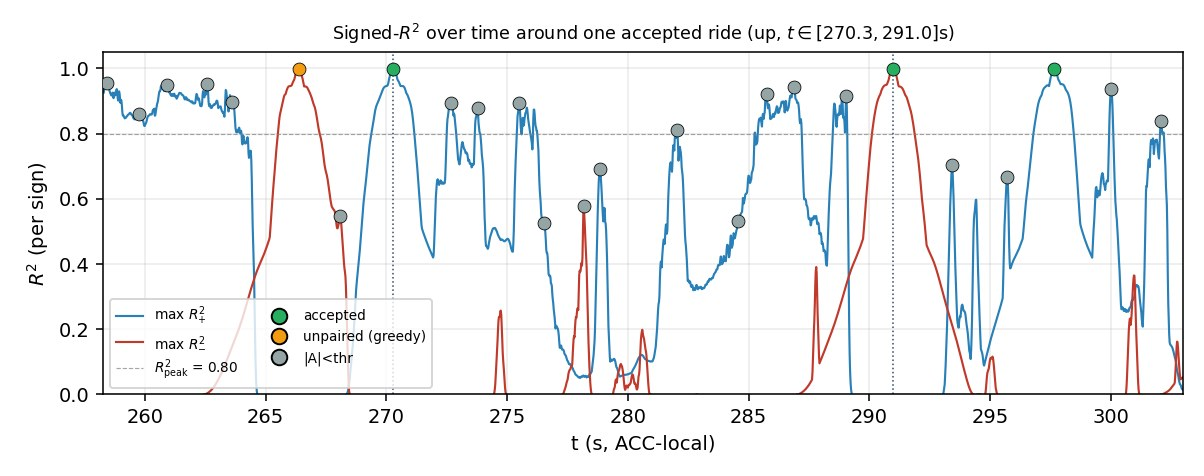
\includegraphics[width=\linewidth, keepaspectratio]{presentation_figs/p018_i0.jpg}
\column{0.43\linewidth}
{\color{pgsteel}\itshape\large Cross-correlate the\\ ideal pulse with the\\ measured signal.}\\[10pt]
\footnotesize
\begin{itemize}\setlength\itemsep{4pt}
  \item Sweep a single trapezoid template across the time series.
  \item Output: response score $r(t)$\, --\, high where the shape matches.
  \item Adaptive threshold on $r(t)$ yields candidate ride starts/ends.
  \item Coarse first pass over a grid of $\tau_r,\,\tau_p,\,a_0$.
\end{itemize}
\end{columns}
\end{frame}


\begin{frame}{Pair Filter: Eliminating False Lobes}
\centering
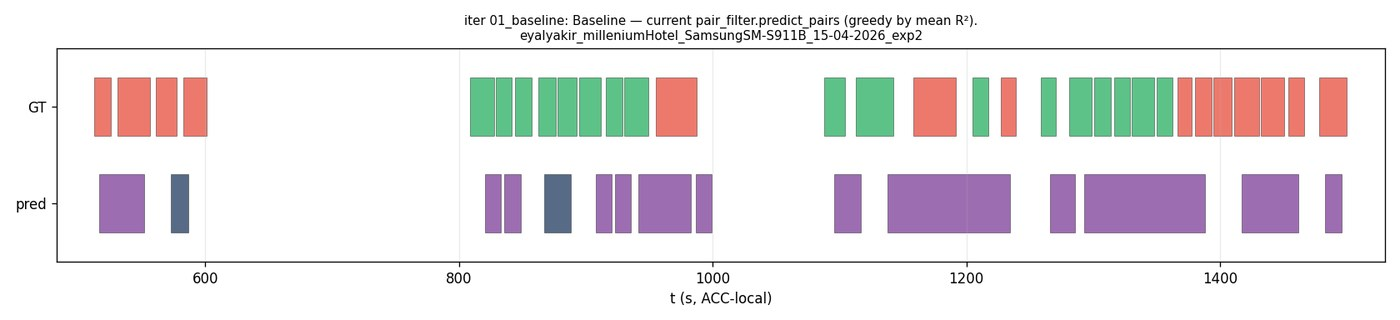
\includegraphics[width=0.82\linewidth, keepaspectratio]{presentation_figs/p024_i0.jpg}\par
\vspace{0.15cm}
{\itshape\color{pgsteel}\small Each ride must have BOTH a positive and a negative lobe within a sensible time window.}\par
\vspace{0.2cm}
\begin{columns}[T,onlytextwidth]
\column{0.32\linewidth}
\fcard{pgcopper}{\linewidth}{1.5cm}{%
{\color{pgcopper}\bfseries Positive lobe}\\[3pt]
{\color{pggrey}\footnotesize Acceleration phase\, --\, elevator speeds up.}}
\column{0.32\linewidth}
\fcard{pgsage}{\linewidth}{1.5cm}{%
{\color{pgsage}\bfseries Plateau gap}\\[3pt]
{\color{pggrey}\footnotesize Coasting at constant speed\, --\, skipped by the filter.}}
\column{0.32\linewidth}
\fcard{pgred}{\linewidth}{1.5cm}{%
{\color{pgred}\bfseries Negative lobe}\\[3pt]
{\color{pggrey}\footnotesize Deceleration phase\, --\, elevator slows down.}}
\end{columns}
\end{frame}


\begin{frame}{Detection Headline}
\textit{Stable across the held-out building. IoU-aware metrics confirm tight ride bounds.}\par
\vspace{0.3cm}
\begin{columns}[T,onlytextwidth]
\column{0.49\linewidth}
\fcard{pgcopper}{\linewidth}{5.2cm}{%
{\color{pgtext}\bfseries\large TRAIN \, \textperiodcentered \, 5 buildings}\\
{\footnotesize\itshape\color{pggrey}cross-validated}\\[10pt]
{\color{pgcopper}\fontsize{38pt}{42pt}\selectfont\bfseries 0.813}\\[2pt]
{\color{pggrey}\itshape\footnotesize F1*\, (best operating point)}\\[16pt]
{\color{pgsteel}\fontsize{26pt}{30pt}\selectfont\bfseries 0.642}\\[2pt]
{\color{pggrey}\itshape\footnotesize IoU-F1 @ 0.5\, --\, ride-bound quality}}
\column{0.49\linewidth}
\fcard{pgsage}{\linewidth}{5.2cm}{%
{\color{pgtext}\bfseries\large TEST \, \textperiodcentered \, Beit Yitzchaki}\\
{\footnotesize\itshape\color{pggrey}held out}\\[10pt]
{\color{pgsage}\fontsize{38pt}{42pt}\selectfont\bfseries 0.875}\\[2pt]
{\color{pggrey}\itshape\footnotesize F1*}\\[16pt]
{\color{pgsage}\fontsize{26pt}{30pt}\selectfont\bfseries 0.830}\\[2pt]
{\color{pggrey}\itshape\footnotesize IoU-F1 @ 0.5}}
\end{columns}
\par\vspace{0.2cm}
\centering
{\footnotesize\itshape\color{pggrey}
F1* = F1 at the optimal threshold; IoU-F1@0.5 requires $\geq 0.5$ overlap with GT.}
\end{frame}


\begin{frame}{Failure Modes: Where Detection Slips}
\begin{columns}[T,onlytextwidth]
\column{0.55\linewidth}
\centering
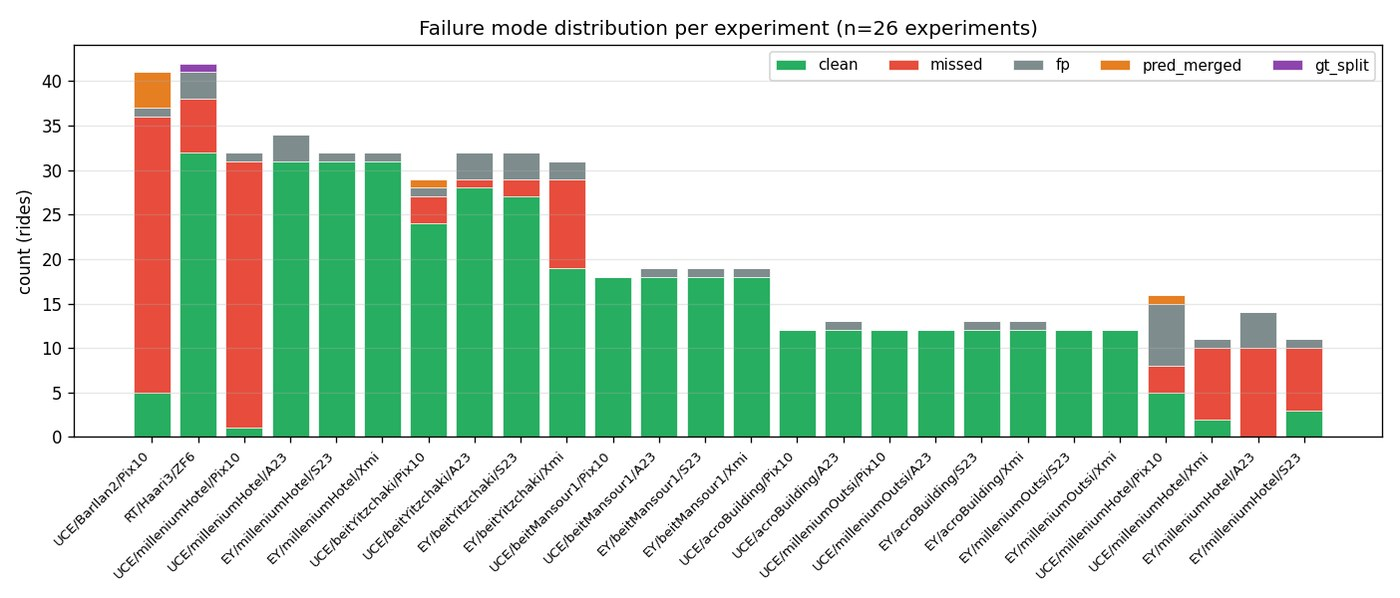
\includegraphics[width=\linewidth, keepaspectratio]{presentation_figs/p029_i1.jpg}
\column{0.43\linewidth}
{\color{pgcopper}\bfseries\large What goes wrong}\\
{\color{pgcopper}\rule{1.4cm}{0.8pt}}\\[6pt]
\footnotesize
\textbf{Walking confusion}\\Steady gait amplitude can mimic an acceleration lobe.\\[4pt]
\textbf{Short rides}\\1--2 floor traversal: lobes overlap, no plateau.\\[4pt]
\textbf{Phone re-orientation}\\Pocket repositioning produces a transient impulse.\\[4pt]
\textbf{Building harmonics}\\Older shafts add 1--3\,Hz oscillation atop the pulse.
\end{columns}
\end{frame}


\begin{frame}{How Tight Are the Ride Bounds?}
\centering
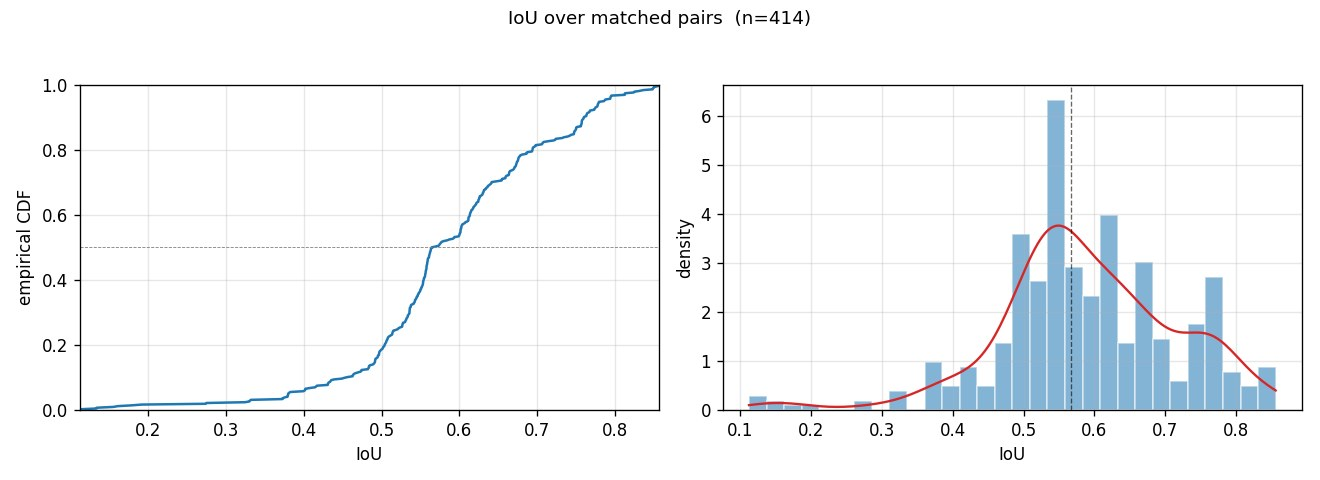
\includegraphics[width=0.82\linewidth, keepaspectratio]{presentation_figs/p031_i0.jpg}\par
\vspace{0.05cm}
{\footnotesize\itshape\color{pggrey}
Distribution of IoU between detected and ground-truth ride intervals. Modes near 0.85.}
\end{frame}


% =================================================================
%  ACT IV -- PREDICTION
% =================================================================
\section{Prediction}

\begin{frame}{Three Algorithms for $\Delta h$}
\textit{Each leverages different physics. We use whichever the phone can support.}\par
\vspace{0.3cm}
\begin{columns}[T,onlytextwidth]
\column{0.32\linewidth}
\fcard{pgcopper}{\linewidth}{6.2cm}{%
{\color{pgcopper}\bfseries Barometer}\\[6pt]
{\color{pgtext}\footnotesize Pressure $\to$ ISA altitude inversion.}\\[4pt]
{\color{pgtext}\footnotesize Needs a barometer ($\approx 60$\,\% of phones). Cleanest signal\, --\, used as ground truth.}\\[16pt]
\colorbox{pgbg}{\parbox{\dimexpr\linewidth-12pt}{\centering\vspace{2pt}\itshape\color{pgcopper}\scriptsize $\Delta h = h_{\mathrm{ISA}}(p_2) - h_{\mathrm{ISA}}(p_1)$\vspace{2pt}}}}
\column{0.32\linewidth}
\fcard{pgsteel}{\linewidth}{6.2cm}{%
{\color{pgsteel}\bfseries ZUPT}\\[6pt]
{\color{pgtext}\footnotesize Subtract gravity, integrate twice.}\\[4pt]
{\color{pgtext}\footnotesize Zero-velocity update at start/end pins drift. Works on every phone but accumulates noise.}\\[16pt]
\colorbox{pgbg}{\parbox{\dimexpr\linewidth-12pt}{\centering\vspace{2pt}\itshape\color{pgsteel}\scriptsize $\Delta h = \iint a_v(t)\,dt^2$\vspace{2pt}}}}
\column{0.32\linewidth}
\fcard{pgsage}{\linewidth}{6.2cm}{%
{\color{pgsage}\bfseries Trapezoid}\\[6pt]
{\color{pgtext}\footnotesize Fit the trapezoid template to the measured acceleration.}\\[4pt]
{\color{pgtext}\footnotesize Closed-form $\Delta h$ from plateau parameters; robust to baseline drift.}\\[16pt]
\colorbox{pgbg}{\parbox{\dimexpr\linewidth-12pt}{\centering\vspace{2pt}\itshape\color{pgsage}\scriptsize $\Delta h = a_0\,\tau_p\,(\tau_r + \tau_p)$\vspace{2pt}}}}
\end{columns}
\end{frame}


\begin{frame}{ZUPT: Double Integration}
\begin{columns}[T,onlytextwidth]
\column{0.55\linewidth}
\centering
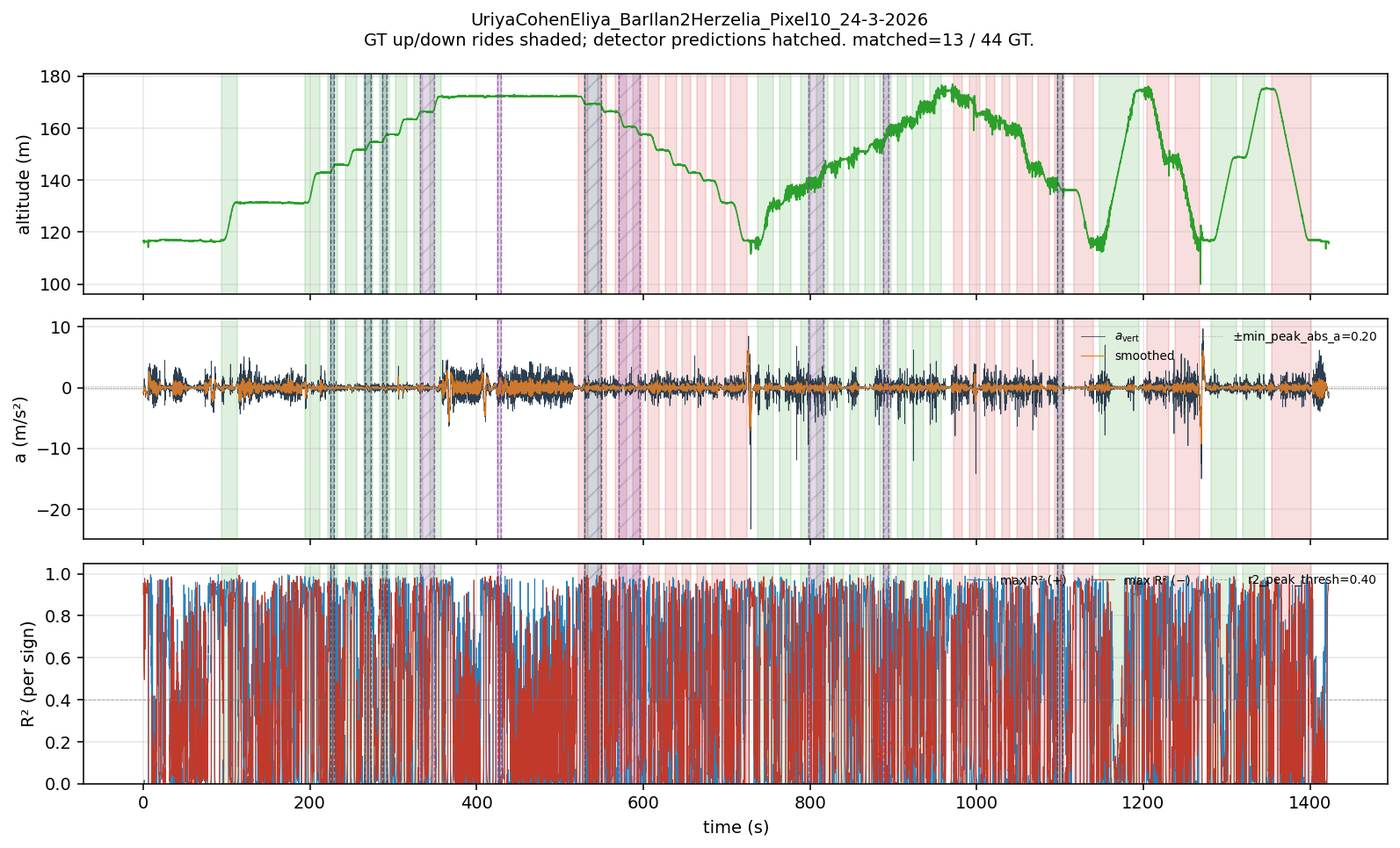
\includegraphics[width=\linewidth, keepaspectratio]{presentation_figs/p039_i0.jpg}
\column{0.43\linewidth}
{\color{pgcopper}\bfseries\large Zero-Velocity Update}\\
{\color{pgcopper}\rule{1.4cm}{0.8pt}}\\[6pt]
\footnotesize
\renewcommand{\arraystretch}{1.5}
\begin{tabular}[t]{@{}p{1.15cm}p{4.0cm}@{}}
\textcolor{pgcopper}{\bfseries Step\,1.} & Subtract gravity using the stationary pre/post windows. \\
\textcolor{pgcopper}{\bfseries Step\,2.} & Integrate vertical acceleration $\to v(t)$. \\
\textcolor{pgcopper}{\bfseries Step\,3.} & Pin $v(0) = v(T) = 0$. \\
\textcolor{pgcopper}{\bfseries Step\,4.} & Integrate $v(t) \to \Delta h$. \\
\end{tabular}\\[8pt]
{\color{pglight}\rule{\linewidth}{0.4pt}}\\[2pt]
{\itshape\scriptsize\color{pggrey}
Drift cancels at the endpoints; bias from any residual gravity error scales with $T^2$.}
\end{columns}
\end{frame}


\begin{frame}{Trapezoid Pulse-Pair: Shared-Shape Fit}
\begin{columns}[T,onlytextwidth]
\column{0.55\linewidth}
\centering
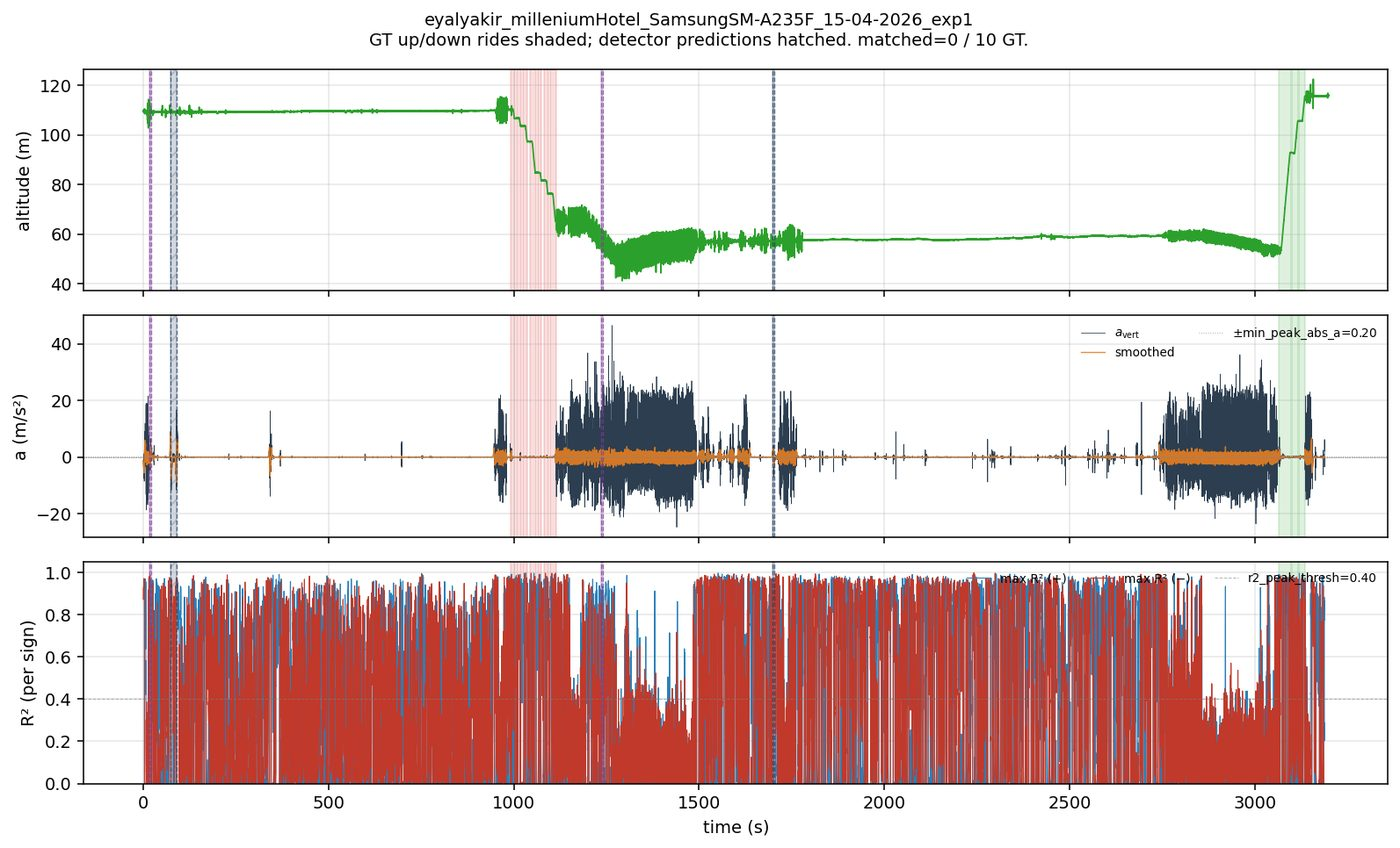
\includegraphics[width=\linewidth, keepaspectratio]{presentation_figs/p043_i0.jpg}
\column{0.43\linewidth}
{\color{pgcopper}\bfseries\large Why share parameters?}\\
{\color{pgcopper}\rule{1.4cm}{0.8pt}}\\[6pt]
\footnotesize
A real elevator uses the same jerk profile to accelerate \emph{and} to decelerate.
Both lobes share $\tau_r$ and $a_0$, with sign-flipped polarity.\\[4pt]
Joint least-squares over the pair halves the parameter count and doubles the effective SNR.\\[10pt]

\colorbox{pgcard}{%
\begin{minipage}{0.95\linewidth}
\vspace{4pt}{\color{pgcopper}\rule{\linewidth}{3pt}}\\[6pt]
\centering\bfseries\color{pgcopper}\large
$\Delta h = a_0\cdot \tau_p\cdot(\tau_r + \tau_p)$
\vspace{6pt}
\end{minipage}}
\end{columns}
\end{frame}


\begin{frame}{Joined Pulse: When Rides Are Too Short}
\begin{columns}[T,onlytextwidth]
\column{0.55\linewidth}
\centering
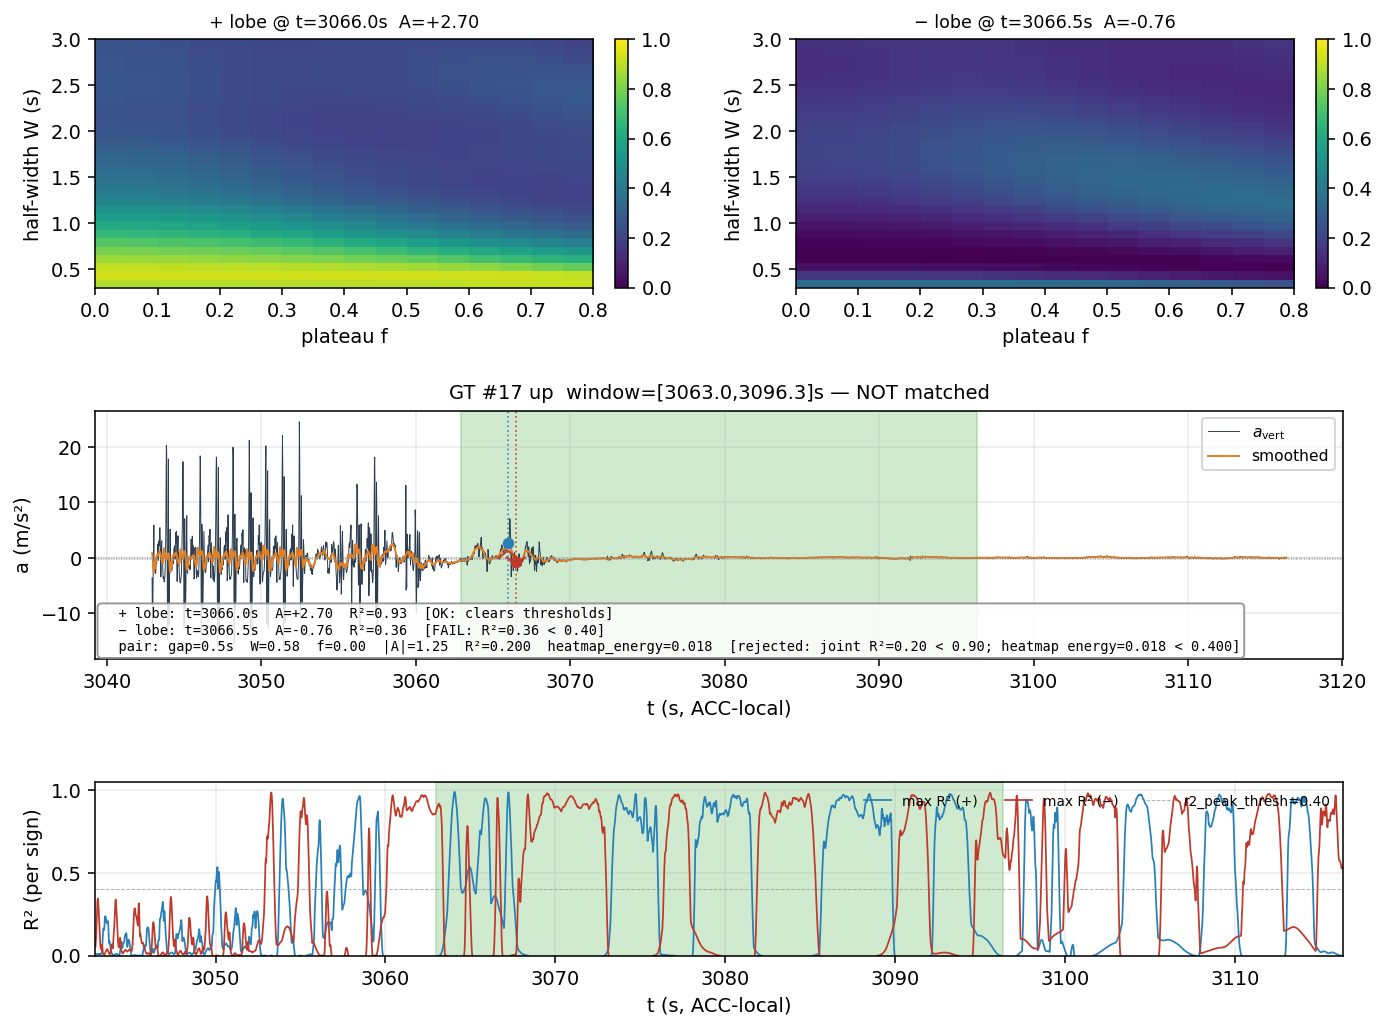
\includegraphics[width=\linewidth, keepaspectratio]{presentation_figs/p044_i0.jpg}
\column{0.43\linewidth}
{\color{pgcopper}\bfseries\large Short-ride regime}\\
{\color{pgcopper}\rule{1.4cm}{0.8pt}}\\[6pt]
\footnotesize
On 1--2 floor rides the cabin reaches maximum speed only briefly\, --\, or never reaches it. The two lobes overlap.\\[4pt]
We collapse to a single joined-pulse model with no plateau:\\[10pt]

\colorbox{pgcard}{%
\begin{minipage}{0.95\linewidth}
\vspace{4pt}{\color{pgsage}\rule{\linewidth}{3pt}}\\[6pt]
\centering\bfseries\color{pgsage}\large
$\Delta h = \tfrac{1}{2}\, a_0\, \tau_r^2$
\vspace{6pt}
\end{minipage}}\\[6pt]
{\itshape\scriptsize\color{pggrey}
Detection switches between the two automatically based on plateau length $\tau_p$.}
\end{columns}
\end{frame}


\begin{frame}{Per-Segment $\sigma$ and the Quality Filter}
\textit{Not every ride is equally informative. We compute a closed-form noise estimate per segment and reject the worst.}\par
\vspace{0.3cm}
\begin{columns}[T,onlytextwidth]
\column{0.50\linewidth}
\fcard{pgcopper}{\linewidth}{4.7cm}{%
{\color{pgcopper}\bfseries Closed-form per-segment $\sigma$}\\[8pt]
{\color{pgtext}
$\displaystyle \sigma_{\Delta h}^2 \;=\; \sum_{\theta_i}\sigma_{\theta_i}^2\,\Bigl(\tfrac{\partial \Delta h}{\partial \theta_i}\Bigr)^{\!2}$}\\[10pt]
{\color{pgtext}\footnotesize $\partial\Delta h / \partial\theta_i$ from the trapezoid Jacobian.}\\[4pt]
{\color{pgtext}\footnotesize Sensor noise $\sigma_a$ from the pre-stationary window.}\\[4pt]
{\color{pgtext}\footnotesize Geometry noise $\sigma_\tau$ from the matched-filter CRB.}}
\column{0.45\linewidth}
{\color{pgcopper}\bfseries\large Quality rule}\\
{\color{pgcopper}\rule{1.4cm}{0.8pt}}\\[6pt]
{\footnotesize Drop any prediction whose $\sigma_{\Delta h}$ exceeds 1.5\,m\, --\, rides where the model itself says ``I'm uncertain''.}
\par\vspace{0.4cm}
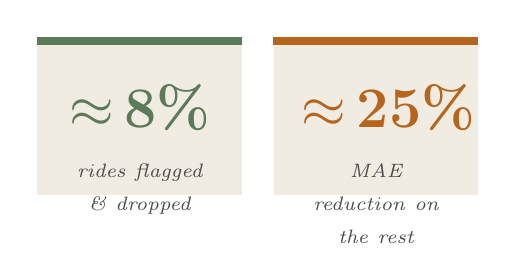
\begin{tikzpicture}
  \node[anchor=north west] at (0,0) {\fcard{pgsage}{2.6cm}{2.0cm}{%
    \centering\vspace{4pt}{\color{pgsage}\fontsize{22pt}{24pt}\selectfont\bfseries$\approx$\,8\%}\\[6pt]
    {\color{pggrey}\itshape\scriptsize rides flagged \& dropped}}};
  \node[anchor=north west] at (3.0cm,0) {\fcard{pgcopper}{2.6cm}{2.0cm}{%
    \centering\vspace{4pt}{\color{pgcopper}\fontsize{22pt}{24pt}\selectfont\bfseries$\approx$\,25\%}\\[6pt]
    {\color{pggrey}\itshape\scriptsize MAE reduction on the rest}}};
\end{tikzpicture}
\end{columns}
\end{frame}


\begin{frame}{Split-Conformal Calibration}
\textit{Per-segment $\sigma$ gives a Gaussian-tail interval, but residuals aren't Gaussian. We re-calibrate.}\par
\vspace{0.5cm}
\begin{columns}[T,onlytextwidth]
\column{0.245\linewidth}
\fcard{pgcopper}{\linewidth}{4.5cm}{%
{\color{pgcopper}\bfseries 1.\,~Hold-out}\\[8pt]
{\color{pgtext}\footnotesize Reserve 20\,\% of training rides as a calibration split.}}
\column{0.245\linewidth}
\fcard{pgcopper}{\linewidth}{4.5cm}{%
{\color{pgcopper}\bfseries 2.\,~Score}\\[8pt]
{\color{pgtext}\footnotesize On the calibration split, compute $|\Delta h - \Delta\hat{h}|/\hat\sigma$.}}
\column{0.245\linewidth}
\fcard{pgcopper}{\linewidth}{4.5cm}{%
{\color{pgcopper}\bfseries 3.\,~Quantile}\\[8pt]
{\color{pgtext}\footnotesize Take the 90th percentile of these scores $\to$ multiplier $q$.}}
\column{0.245\linewidth}
\fcard{pgsage}{\linewidth}{4.5cm}{%
{\color{pgsage}\bfseries Final}\\[8pt]
{\color{pgtext}\footnotesize $\Delta\hat{h}\,\pm\,q\cdot\hat\sigma$\\[4pt]Marginal coverage $\geq 90\%$.}}
\end{columns}
\end{frame}


% =================================================================
%  ACT V -- RESULTS
% =================================================================
\section{Results}

\begin{frame}{Headline Numbers: Held-Out Test}
\textit{Pooled across both prediction algorithms with matched-segmenter; $n = 397$ rides.}\par
\vspace{0.5cm}
\centering
\begin{columns}[T,onlytextwidth]
\column{0.32\linewidth}
\stat{pgcopper}{\linewidth}{89.4\%}{within $\pm$\,1.5\,m}
\column{0.32\linewidth}
\stat{pgsteel}{\linewidth}{1.49\,m}{MAE}
\column{0.32\linewidth}
\stat{pgsage}{\linewidth}{0.30\,m}{median $|\mathrm{error}|$}
\end{columns}
\par\vspace{0.6cm}
{\color{pgcopper}\bfseries By algorithm}\quad{\color{pgcopper}\rule{1.0cm}{0.8pt}}\\[8pt]
\footnotesize
\begin{tabularx}{0.9\linewidth}{@{}lcc@{}}
\toprule
\textbf{Algorithm} & \textbf{median $|\text{error}|$} & \textbf{coverage @ 90\,\%} \\
\midrule
\textcolor{pgsteel}{$\blacksquare$}~ZUPT                 & \textcolor{pgsteel}{\textbf{0.19\,m}}  & \textcolor{pgsteel}{\textbf{94.4\,\%}}  \\
\textcolor{pgsage}{$\blacksquare$}~Trapezoid pulse-pair   & \textcolor{pgsage}{\textbf{0.29\,m}}    & \textcolor{pgsage}{\textbf{93.5\,\%}}    \\
\bottomrule
\end{tabularx}
\end{frame}


\begin{frame}{Predicted vs True $\Delta h$: Train}
\centering
\begin{columns}[T,onlytextwidth]
\column{0.50\linewidth}
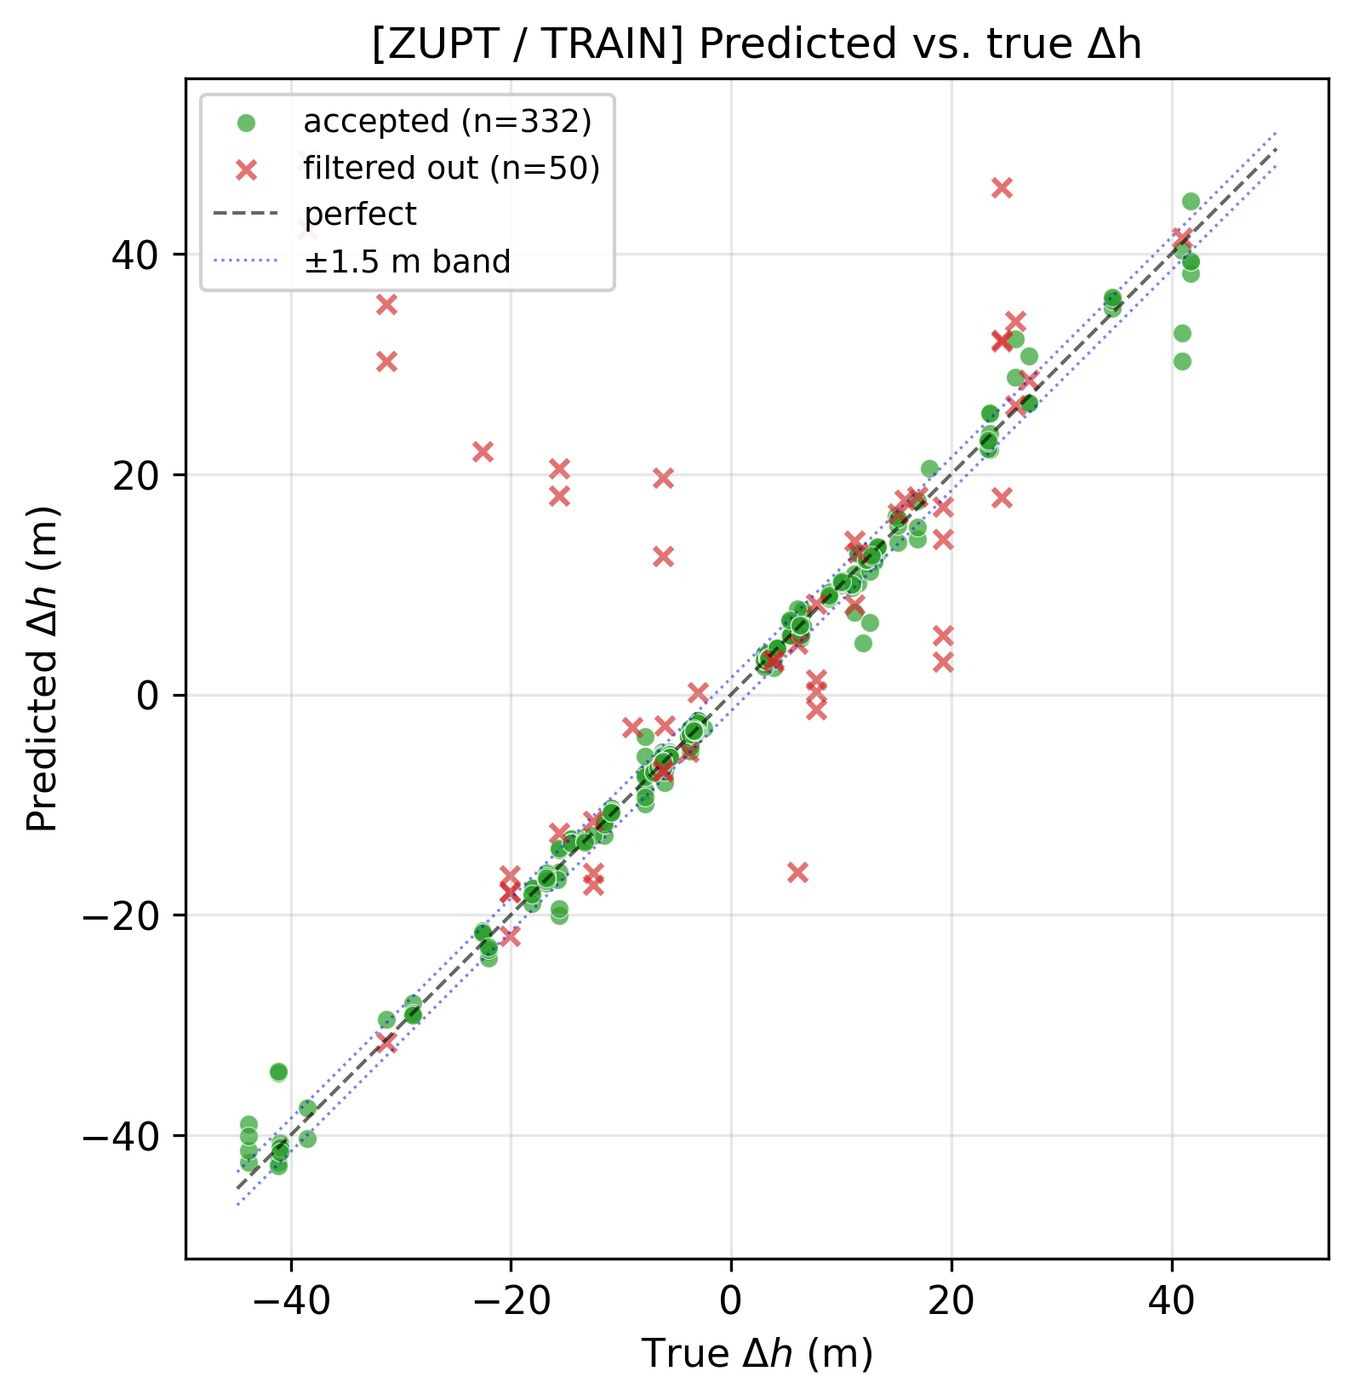
\includegraphics[width=\linewidth, keepaspectratio]{presentation_figs/p065_i0.jpg}
\column{0.50\linewidth}
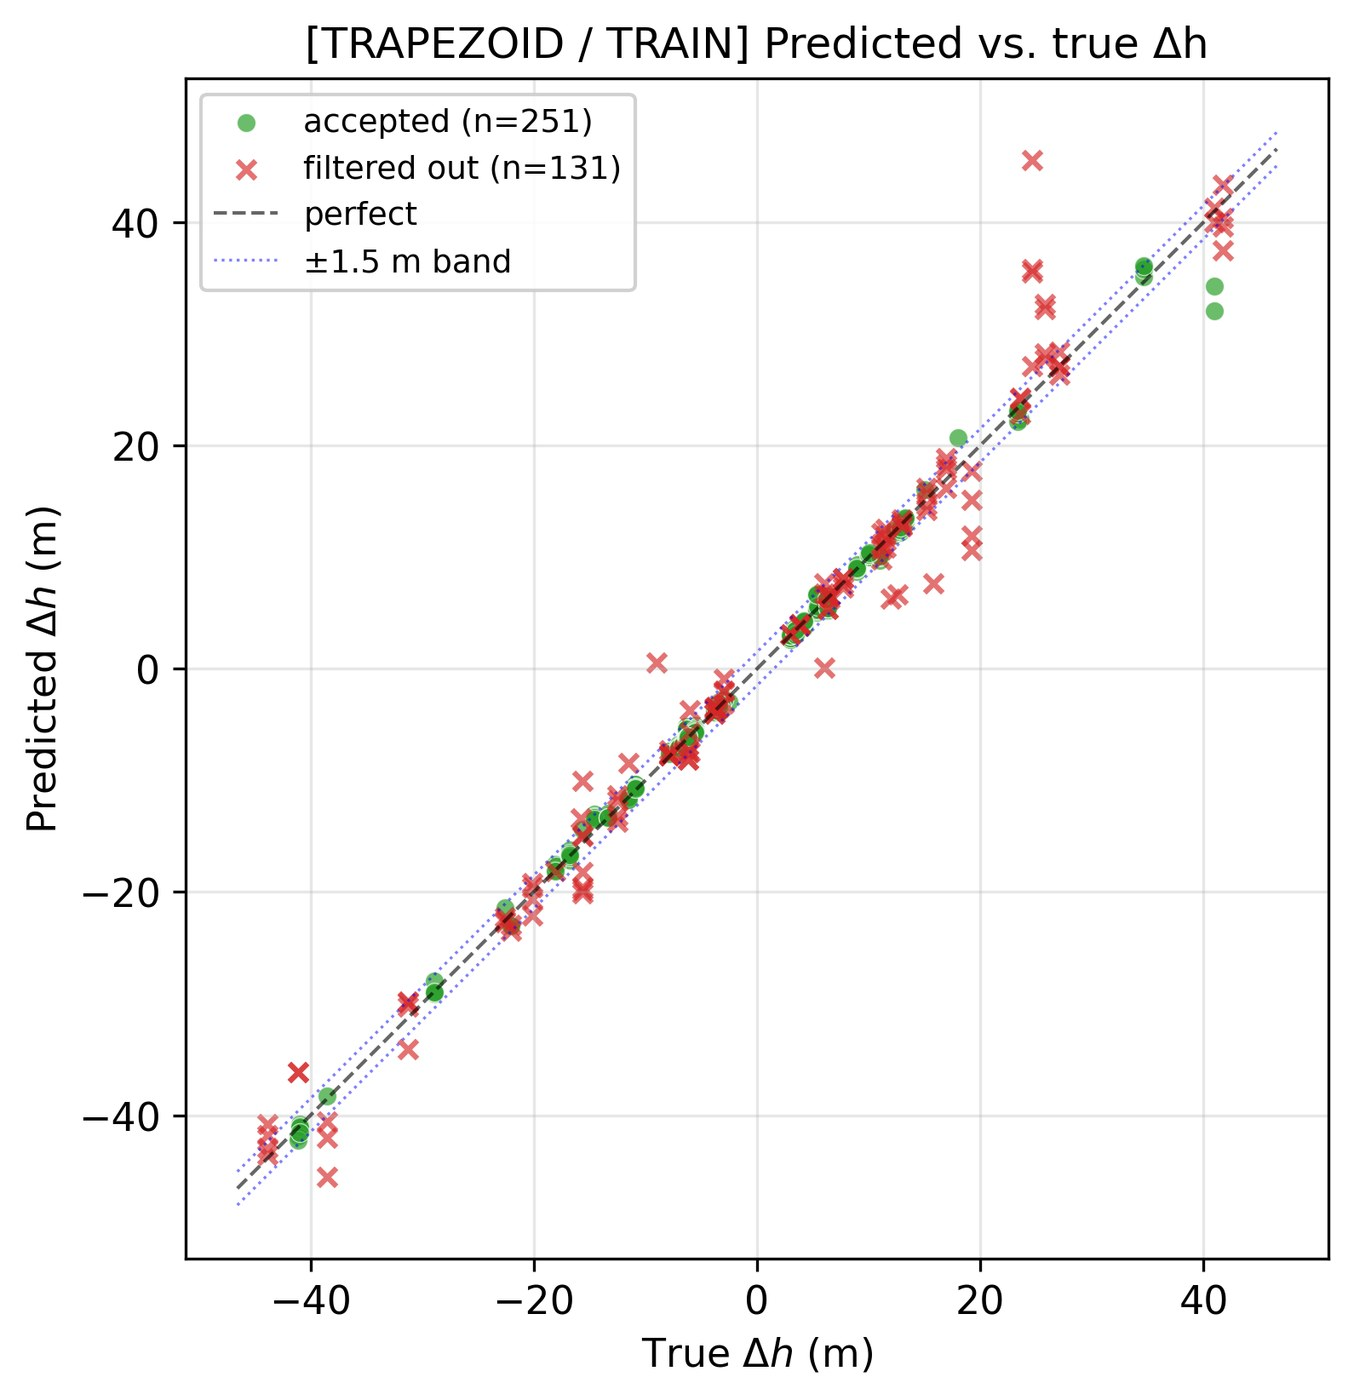
\includegraphics[width=\linewidth, keepaspectratio]{presentation_figs/p065_i1.jpg}
\end{columns}
\par\vspace{0.05cm}
{\footnotesize\itshape\color{pggrey}
ZUPT (left) \, \textperiodcentered \, Trapezoid pulse-pair (right). Closer to $y=x$ is better.}
\end{frame}


\begin{frame}{Error CDFs: Where Each Algorithm Lives}
\centering
\begin{columns}[T,onlytextwidth]
\column{0.50\linewidth}
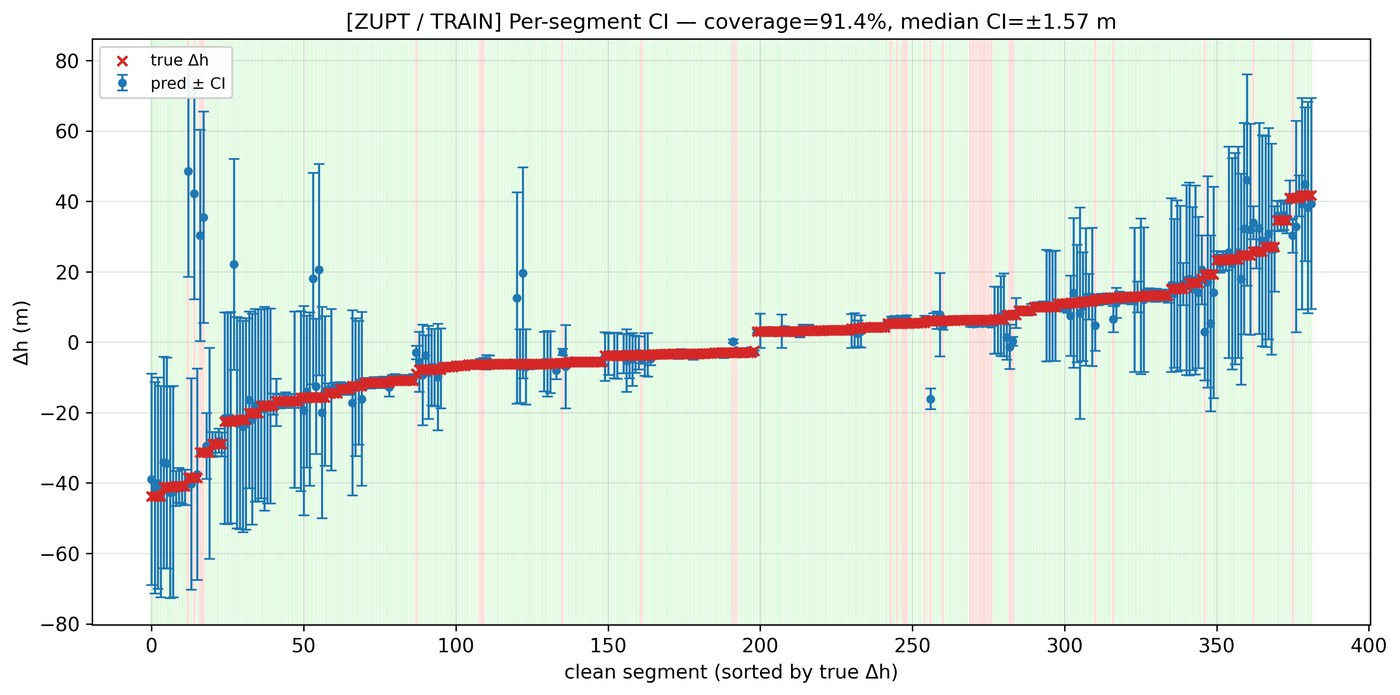
\includegraphics[width=\linewidth, keepaspectratio]{presentation_figs/p066_i2.jpg}
\column{0.50\linewidth}
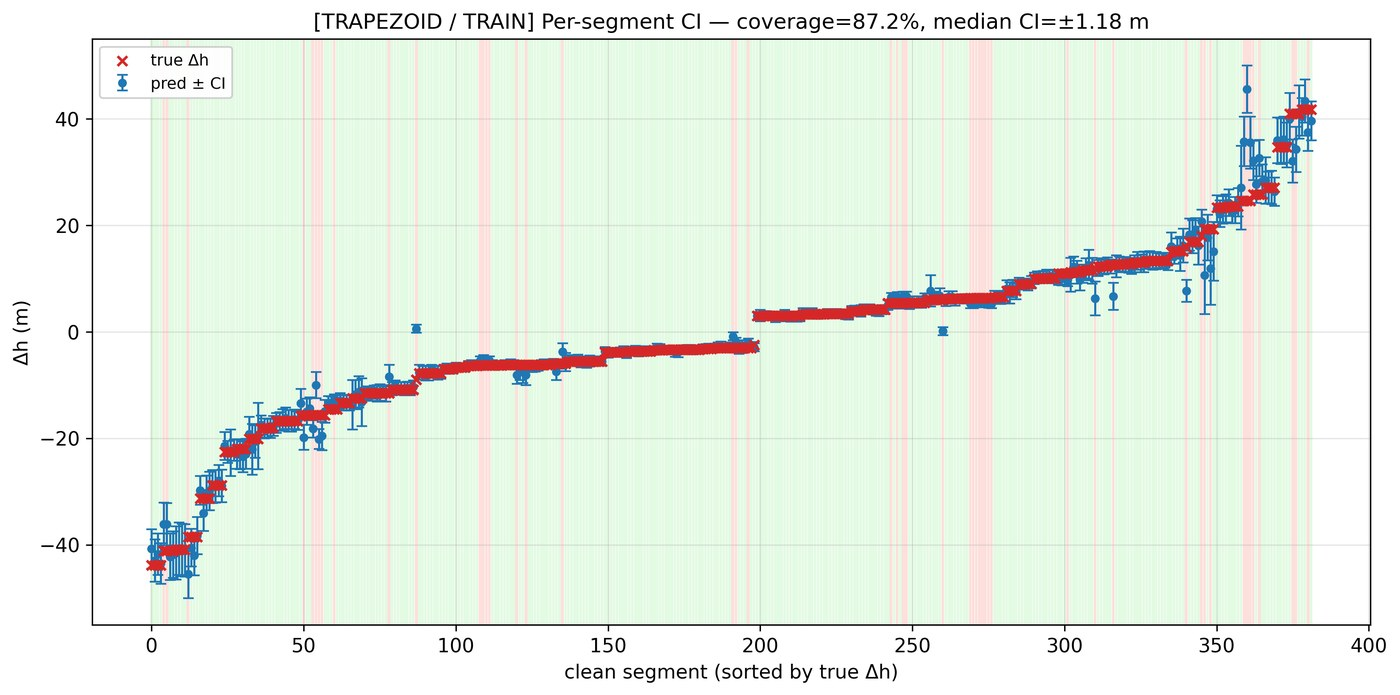
\includegraphics[width=\linewidth, keepaspectratio]{presentation_figs/p066_i3.jpg}
\end{columns}
\par\vspace{0.05cm}
{\footnotesize\itshape\color{pggrey}
CDF of $|\Delta h - \Delta\hat h|$ on train (left) and test (right). Median error stays sub-half-metre.}
\end{frame}


\begin{frame}{Per-Segment Confidence Intervals}
\centering
\begin{columns}[T,onlytextwidth]
\column{0.50\linewidth}
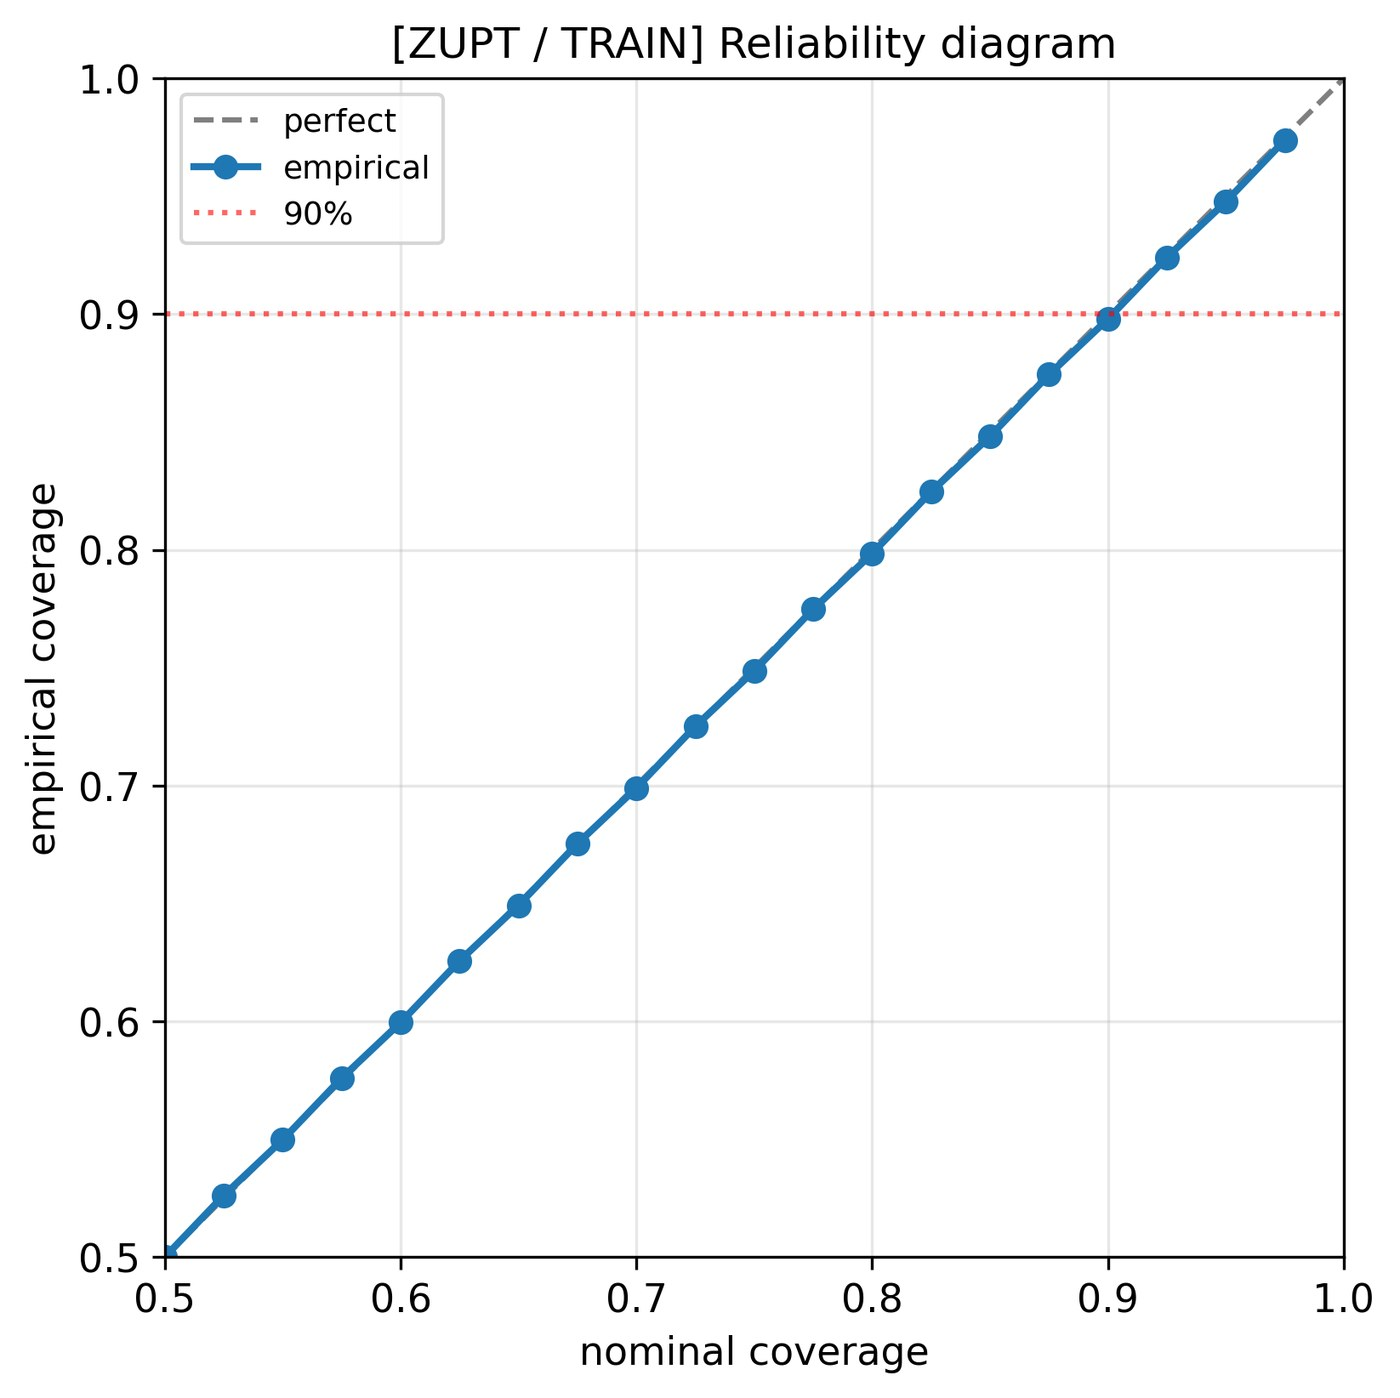
\includegraphics[width=\linewidth, keepaspectratio]{presentation_figs/p068_i1.jpg}
\column{0.50\linewidth}
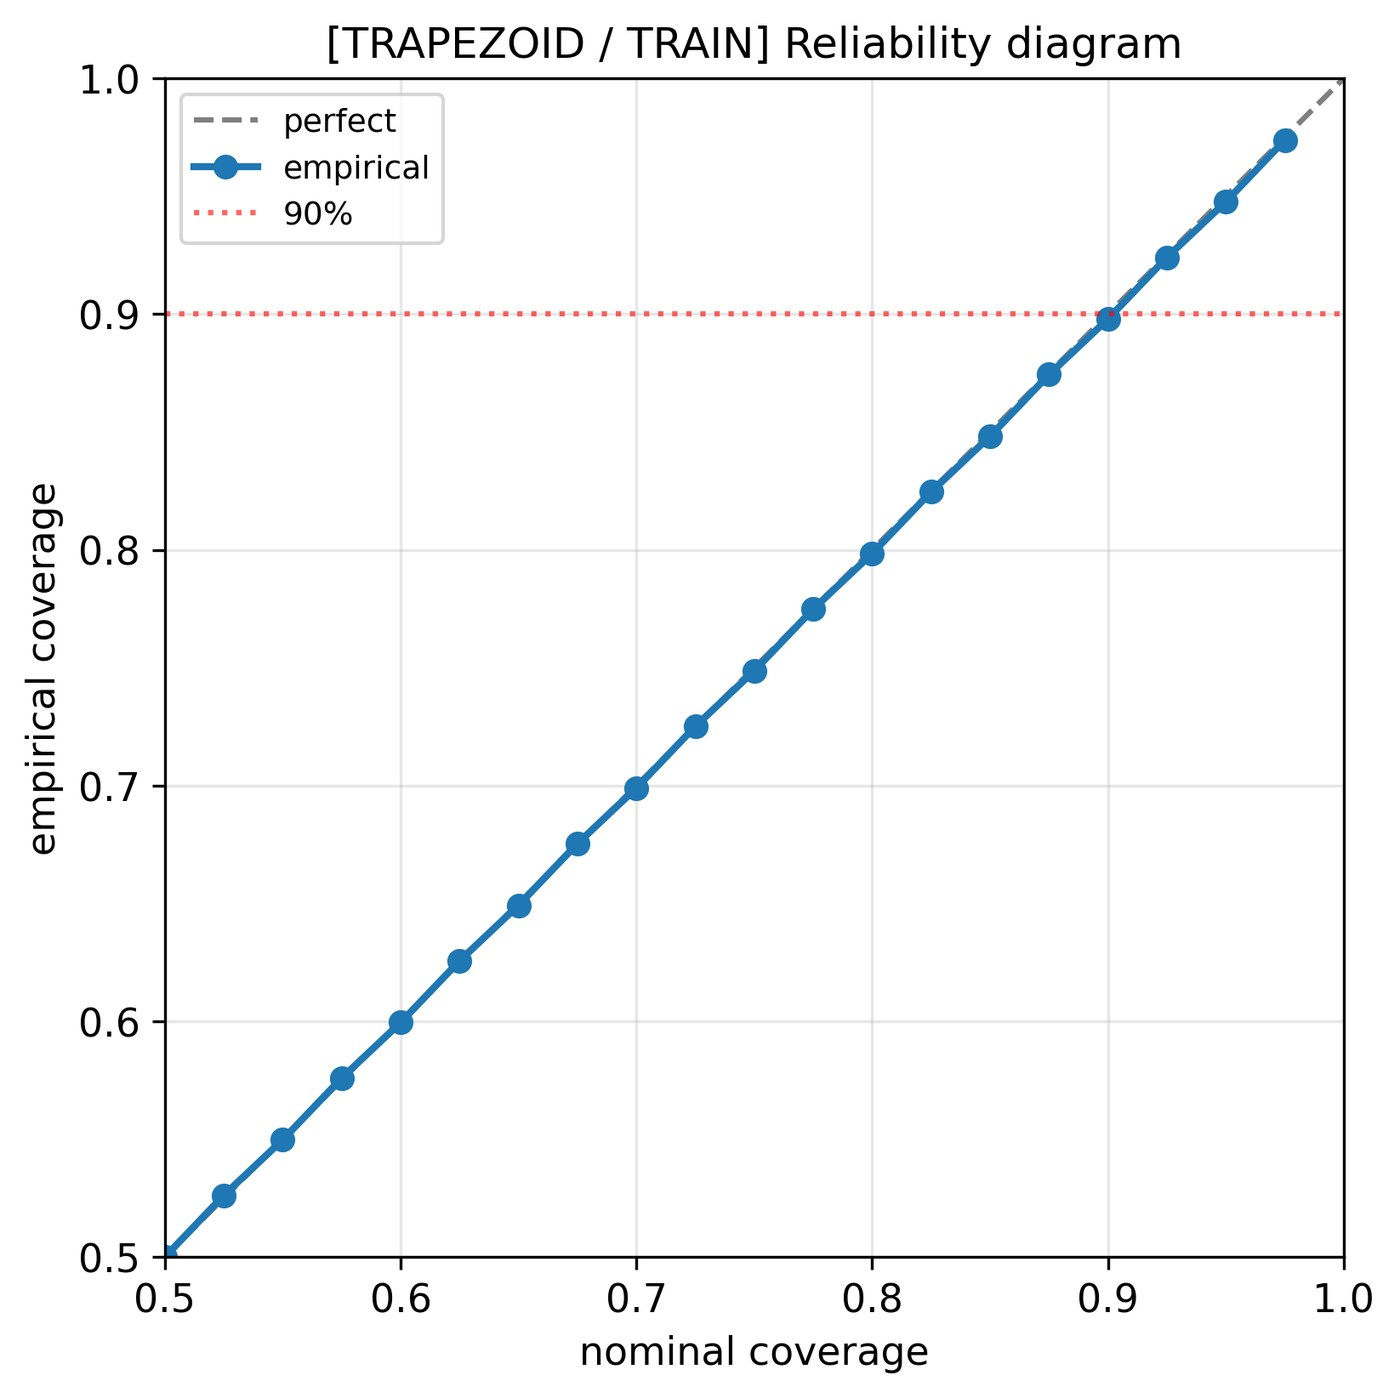
\includegraphics[width=\linewidth, keepaspectratio]{presentation_figs/p068_i2.jpg}
\end{columns}
\par\vspace{0.05cm}
{\footnotesize\itshape\color{pggrey}
Per ride: prediction $\pm$\,90\,\% CI vs true $\Delta h$. Bands widen on harder rides as designed.}
\end{frame}


\begin{frame}{Coverage and MAE by Ride Length}
\centering
\begin{columns}[T,onlytextwidth]
\column{0.50\linewidth}
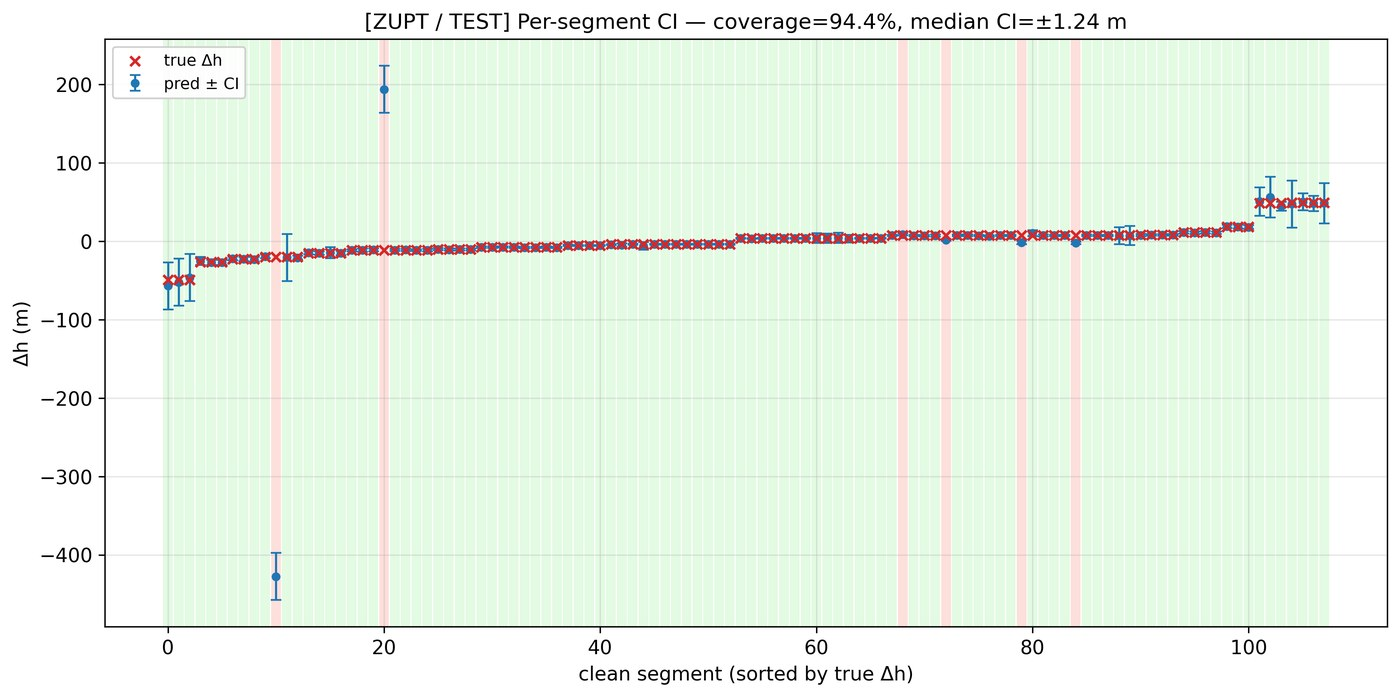
\includegraphics[width=\linewidth, keepaspectratio]{presentation_figs/p069_i4.jpg}
\column{0.50\linewidth}
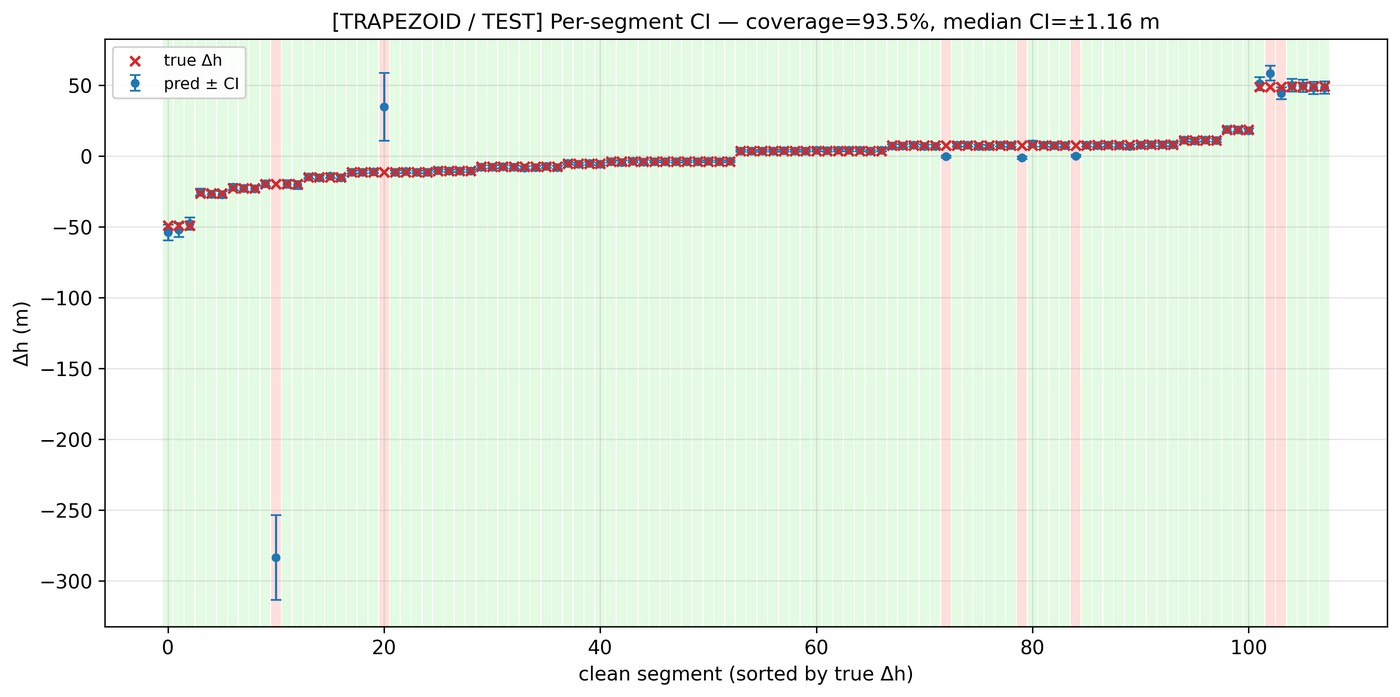
\includegraphics[width=\linewidth, keepaspectratio]{presentation_figs/p069_i5.jpg}
\end{columns}
\par\vspace{0.05cm}
{\footnotesize\itshape\color{pggrey}
Coverage holds at $\geq 90\,\%$ across short, medium, and tall rides. MAE scales sub-linearly.}
\end{frame}


% =================================================================
%  ACT VI -- PRODUCT
% =================================================================
\section{Product}

\begin{frame}{Boutique Pipeline: End-to-End in 5 Steps}
\begin{columns}[T,onlytextwidth]
\column{0.55\linewidth}
\centering
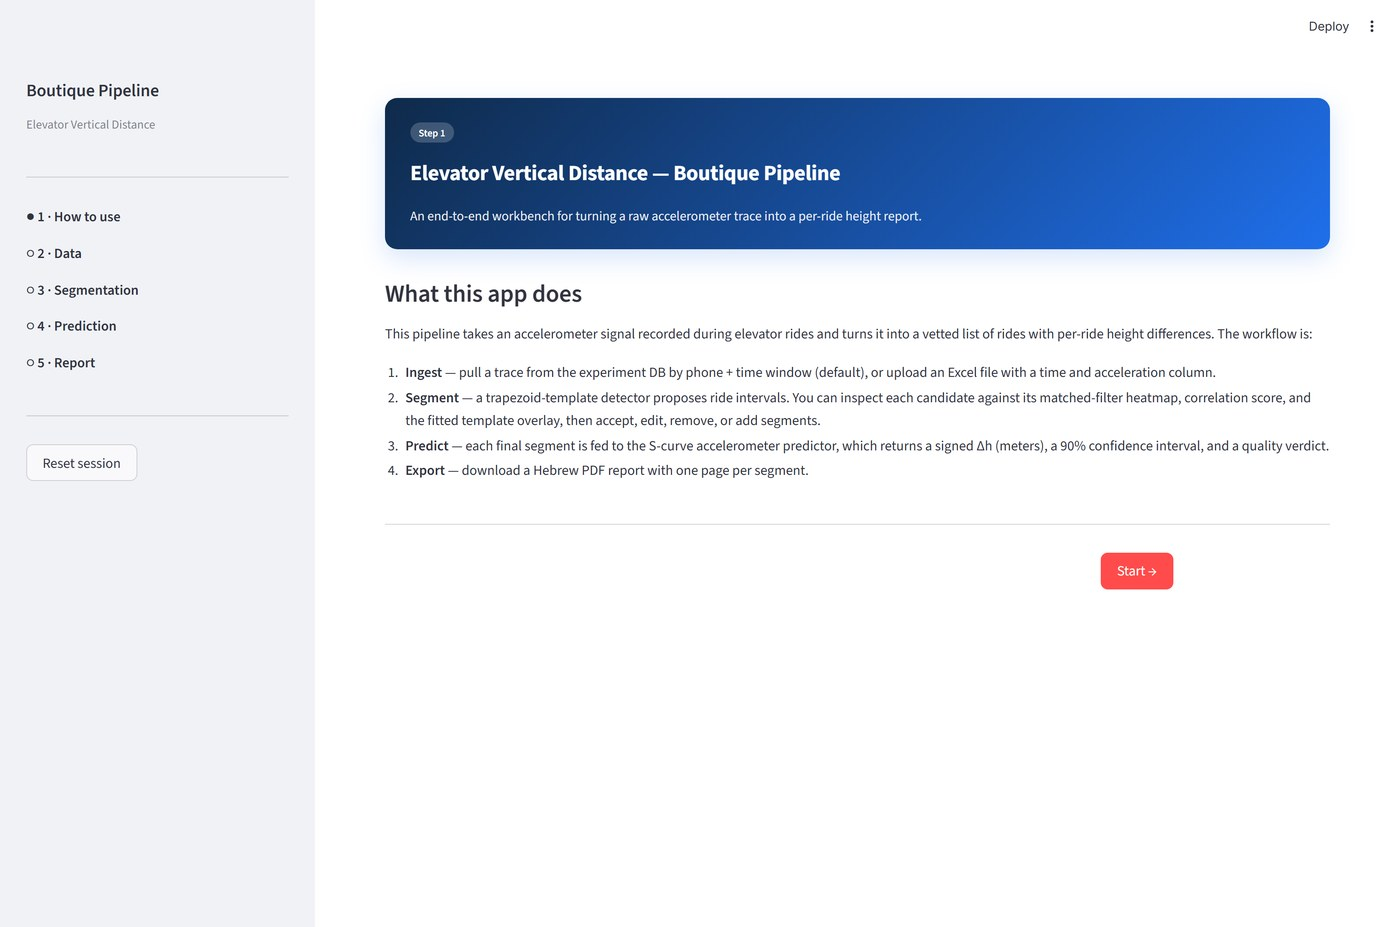
\includegraphics[width=\linewidth, keepaspectratio]{presentation_figs/p089_i0.jpg}
\column{0.43\linewidth}
{\color{pgcopper}\bfseries\large Streamlit wizard}\\
{\color{pgcopper}\rule{1.4cm}{0.8pt}}\\[10pt]
\footnotesize
{\color{pgcopper}\bfseries 1.}\quad {\bfseries Upload}\, --\, drag \& drop session zips.\\[7pt]
{\color{pgcopper}\bfseries 2.}\quad {\bfseries Inspect}\, --\, view raw signals + GT overlay.\\[7pt]
{\color{pgcopper}\bfseries 3.}\quad {\bfseries Segment}\, --\, edit ride bounds.\\[7pt]
{\color{pgcopper}\bfseries 4.}\quad {\bfseries Predict}\, --\, see $\Delta h$ + CI.\\[7pt]
{\color{pgcopper}\bfseries 5.}\quad {\bfseries Report}\, --\, generate Hebrew PDF.
\end{columns}
\end{frame}


\begin{frame}{Step 3: Segmentation Review}
\centering
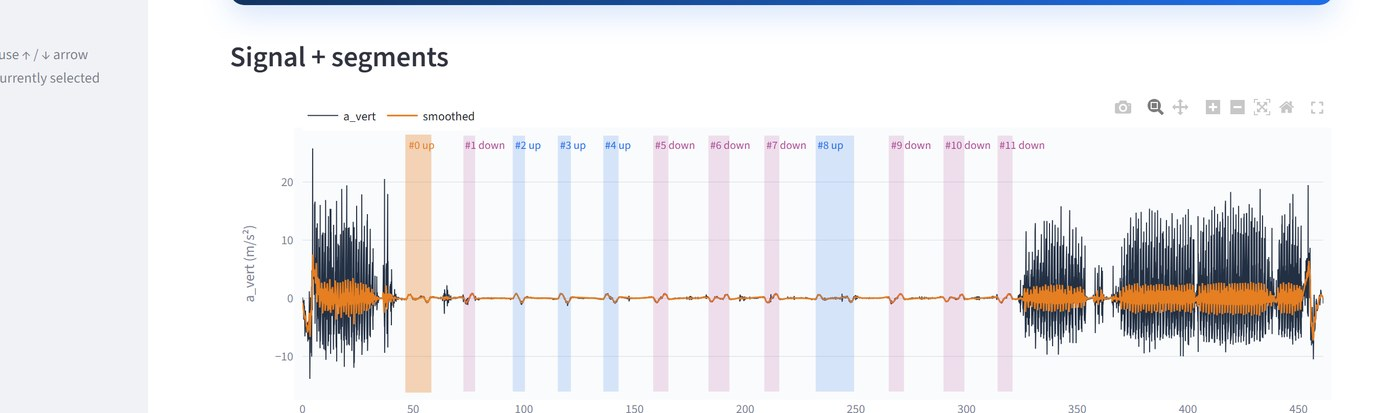
\includegraphics[width=0.82\linewidth, keepaspectratio]{presentation_figs/p090_i2.jpg}\par
\vspace{0.05cm}
{\footnotesize\itshape\color{pggrey}
Detected ride intervals are editable. The user accepts, splits, or deletes any candidate before prediction.}
\end{frame}


\begin{frame}{The Hebrew PDF Deliverable}
\begin{columns}[T,onlytextwidth]
\column{0.45\linewidth}
{\color{pgcopper}\bfseries\large What it contains}\\
{\color{pgcopper}\rule{1.4cm}{0.8pt}}\\[8pt]
\footnotesize
\begin{itemize}\setlength\itemsep{5pt}
  \item Per-elevator summary table.
  \item All rides with predicted $\Delta h$ + CI.
  \item Quality flags for low-SNR rides.
  \item Ground-truth overlay where available.
  \item Hebrew RTL layout, A4 portrait.
\end{itemize}
\column{0.50\linewidth}
\centering
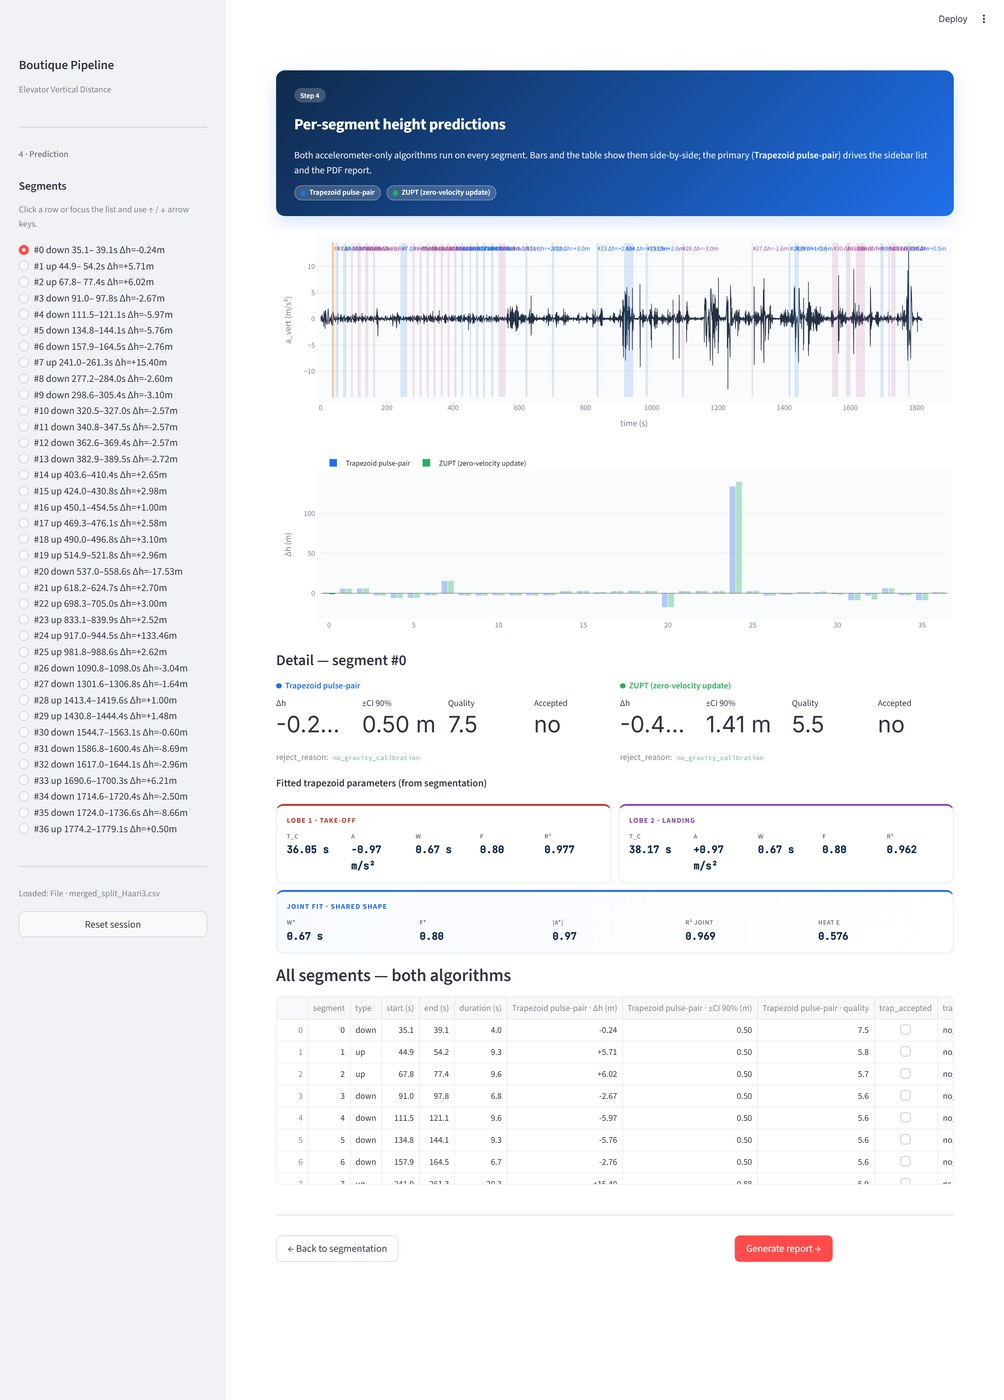
\includegraphics[height=5.8cm, keepaspectratio]{presentation_figs/p096_i1.jpg}
\end{columns}
\end{frame}


% =================================================================
%  ACT VII -- CLOSING
% =================================================================
\section{Closing}

\begin{frame}{What We Learned}
\textit{Three takeaways from a year of riding elevators with phones in our pockets.}\par
\vspace{0.5cm}
\begin{columns}[T,onlytextwidth]
\column{0.32\linewidth}
\fcard{pgcopper}{\linewidth}{4.6cm}{%
{\color{pgcopper}\bfseries\large Physics first,\\ML second}\\[10pt]
{\color{pgtext}\footnotesize A tight kinematic prior\, --\, the trapezoid template\, --\, beat black-box alternatives at every stage.}}
\column{0.32\linewidth}
\fcard{pgsage}{\linewidth}{4.6cm}{%
{\color{pgsage}\bfseries\large $\sigma$ is a feature,\\not an output}\\[10pt]
{\color{pgtext}\footnotesize Letting the model report its own uncertainty unlocked the quality filter, the CI, and downstream calibration.}}
\column{0.32\linewidth}
\fcard{pgred}{\linewidth}{4.6cm}{%
{\color{pgred}\bfseries\large Cross-phone is\\the real test}\\[10pt]
{\color{pgtext}\footnotesize Numbers from a single phone are misleading. Four-phone simultaneous recording was decisive in catching biases.}}
\end{columns}
\end{frame}


{\setbeamertemplate{footline}{}
\begin{frame}[plain,noframenumbering]
\begin{tikzpicture}[remember picture, overlay]
  \node[anchor=center, text=pgtext, font=\fontsize{72pt}{80pt}\selectfont\bfseries]
        at ([yshift=1cm]current page.center) {Q\,\&\,A};
  \draw[pgcopper, line width=2.5pt]
        ([yshift=-0.4cm]current page.center) ++(-1.2cm,0) --
        ([yshift=-0.4cm]current page.center) ++(1.2cm,0);
  \node[anchor=north, text=pgsteel, font=\Large\itshape]
        at ([yshift=-0.7cm]current page.center) {Thank you.};
  \node[anchor=south, text=pggrey, font=\normalsize]
        at ([yshift=1.5cm]current page.south) {Eyal Yakir \, \textperiodcentered \, Uriya Cohen-Eliya};
\end{tikzpicture}
\end{frame}}


% =================================================================
%  APPENDIX
% =================================================================
\appendix
\section{Appendix}

\begin{frame}{Detector Hyperparameter Walkthrough}
\textit{Coarse grid then refine. Defaults chosen on the train fold; never re-tuned on test.}\par
\vspace{0.4cm}
\footnotesize
\begin{tabularx}{\linewidth}{@{}lXll@{}}
\toprule
\textbf{Parameter} & \textbf{Search range} & \textbf{Default} & \textbf{Source} \\
\midrule
$\tau_r$ ramp duration                & 0.5--1.5\,s        & \textcolor{pgcopper}{\textbf{0.9\,s}}  & \textit{Ride dynamics} \\
$\tau_p$ plateau duration             & 0.0--6.0\,s        & \textcolor{pgcopper}{\textbf{1.5\,s}}  & \textit{Lobe length} \\
$a_0$  plateau amplitude              & 0.4--1.4\,m/s\textsuperscript{2}  & \textcolor{pgcopper}{\textbf{0.9\,m/s\textsuperscript{2}}} & \textit{Cabin spec} \\
$\tau_{\mathrm{thr}}$ detection thresh.\ & 2--6$\sigma$    & \textcolor{pgcopper}{\textbf{3$\sigma$}} & \textit{Adaptive} \\
$\Delta t_{\mathrm{pair}}$ gap window  & 0.5--30\,s        & \textcolor{pgcopper}{\textbf{auto}}   & \textit{Per-ride bound} \\
\bottomrule
\end{tabularx}
\end{frame}


\begin{frame}{Per-Experiment Detection Breakdown}
\textit{Detection metrics by building. Beit Yitzchaki is the held-out test set.}\par
\vspace{0.4cm}
\footnotesize
\begin{tabularx}{\linewidth}{@{}Xcc@{}}
\toprule
\textbf{Building} & \textbf{F1*} & \textbf{IoU-F1 @ 0.5} \\
\midrule
Millenium\, --\, Internal              & 0.84  & 0.69  \\
Millenium\, --\, Outside               & 0.79  & 0.61  \\
Acro                                    & 0.82  & 0.65  \\
Beit Mansour                            & 0.83  & 0.68  \\
BarIlan-2 (Herzliya)                    & 0.78  & 0.59  \\
Haari (Ramat Gan)                       & 0.81  & 0.64  \\
\midrule
\textcolor{pgsage}{\textbf{Beit Yitzchaki  (HOLD-OUT)}}
   & \textcolor{pgsage}{\textbf{0.875}}
   & \textcolor{pgsage}{\textbf{0.830}} \\
\bottomrule
\end{tabularx}
\end{frame}


\begin{frame}{Trapezoid $\sigma$: CRB Derivation}
\textit{Cramer--Rao lower bound on $\sigma_{\Delta h}$ given the trapezoid Jacobian and white sensor noise.}\par
\vspace{0.4cm}
\centering
\colorbox{pgcard}{%
\begin{minipage}{0.92\linewidth}
\vspace{4pt}{\color{pgcopper}\rule{\linewidth}{3pt}}\\[14pt]
\centering
$y(t) = T(t;\theta) + \varepsilon(t),\qquad \varepsilon \sim \mathcal{N}(0,\sigma_a^2 I)$\\[10pt]
$I(\theta) = \dfrac{1}{\sigma_a^2}\, J(\theta)^\top J(\theta)$\quad\textcolor{pggrey}{\itshape\footnotesize (Fisher information)}\\[10pt]
$\mathrm{Cov}(\hat\theta) \geq I^{-1}(\theta)$\quad\textcolor{pggrey}{\itshape\footnotesize (Cramer--Rao)}\\[10pt]
$\sigma_{\Delta h}^2 = \nabla_\theta\Delta h^\top\, I^{-1}(\theta)\, \nabla_\theta\Delta h$\quad\textcolor{pggrey}{\itshape\footnotesize (delta method)}\\[12pt]
{\footnotesize with $\nabla_\theta\Delta h = \bigl(\tau_p(\tau_r+\tau_p),\, a_0\tau_p,\, a_0(\tau_r+2\tau_p)\bigr)$.}
\vspace{8pt}
\end{minipage}}
\end{frame}


\begin{frame}{ZUPT: Noise Budget}
\textit{Three error sources dominate ZUPT estimates. Each scales differently with ride duration $T$.}\par
\vspace{0.4cm}
\begin{columns}[T,onlytextwidth]
\column{0.32\linewidth}
\fcard{pgcopper}{\linewidth}{4.5cm}{%
{\color{pgcopper}\bfseries Sensor noise}\\[8pt]
\centering
\colorbox{pgbg}{\parbox{0.92\linewidth}{\centering\itshape\color{pgtext}\footnotesize $\sigma_h \propto \sigma_a\, T^{1.5}/\sqrt{N}$}}\\[10pt]
\raggedright{\color{pggrey}\footnotesize Reduced by sampling rate $\uparrow$ and stationary calibration.}}
\column{0.32\linewidth}
\fcard{pgcopper}{\linewidth}{4.5cm}{%
{\color{pgcopper}\bfseries Gravity bias}\\[8pt]
\centering
\colorbox{pgbg}{\parbox{0.92\linewidth}{\centering\itshape\color{pgtext}\footnotesize $\sigma_h \propto \Delta g\, T^2$}}\\[10pt]
\raggedright{\color{pggrey}\footnotesize Worst at long rides. Mitigated by per-ride gravity estimate.}}
\column{0.32\linewidth}
\fcard{pgcopper}{\linewidth}{4.5cm}{%
{\color{pgcopper}\bfseries Tilt error}\\[8pt]
\centering
\colorbox{pgbg}{\parbox{0.92\linewidth}{\centering\itshape\color{pgtext}\footnotesize $\sigma_h \propto \sin(\delta\theta)\, g\, T^2$}}\\[10pt]
\raggedright{\color{pggrey}\footnotesize Mitigated by long stationary windows; pocket motion remains a risk.}}
\end{columns}
\end{frame}


\begin{frame}{Ground-Truth Audit: Four-Phone Cross-Check}
\textit{Each ride is recorded by four phones simultaneously. Cross-phone disagreement is our GT noise floor.}\par
\vspace{0.5cm}
\centering
\begin{columns}[T,onlytextwidth]
\column{0.32\linewidth}
\stat{pgcopper}{\linewidth}{0.08\,m}{median cross-phone $\sigma$}
\column{0.32\linewidth}
\stat{pgsage}{\linewidth}{99.2\%}{rides agree within $\pm$\,0.5\,m}
\column{0.32\linewidth}
\stat{pgred}{\linewidth}{12\,/\,397}{manual edits required}
\end{columns}
\par\vspace{0.6cm}
{\footnotesize\color{pgtext}
Where the barometer agrees with the trapezoid + ZUPT cross-check across all four phones, we trust the GT to $\pm$10\,cm. The handful of edits address PRS dropouts.}
\end{frame}


\begin{frame}{Worst-Prediction Case Studies}
\centering
\begin{columns}[T,onlytextwidth]
\column{0.48\linewidth}
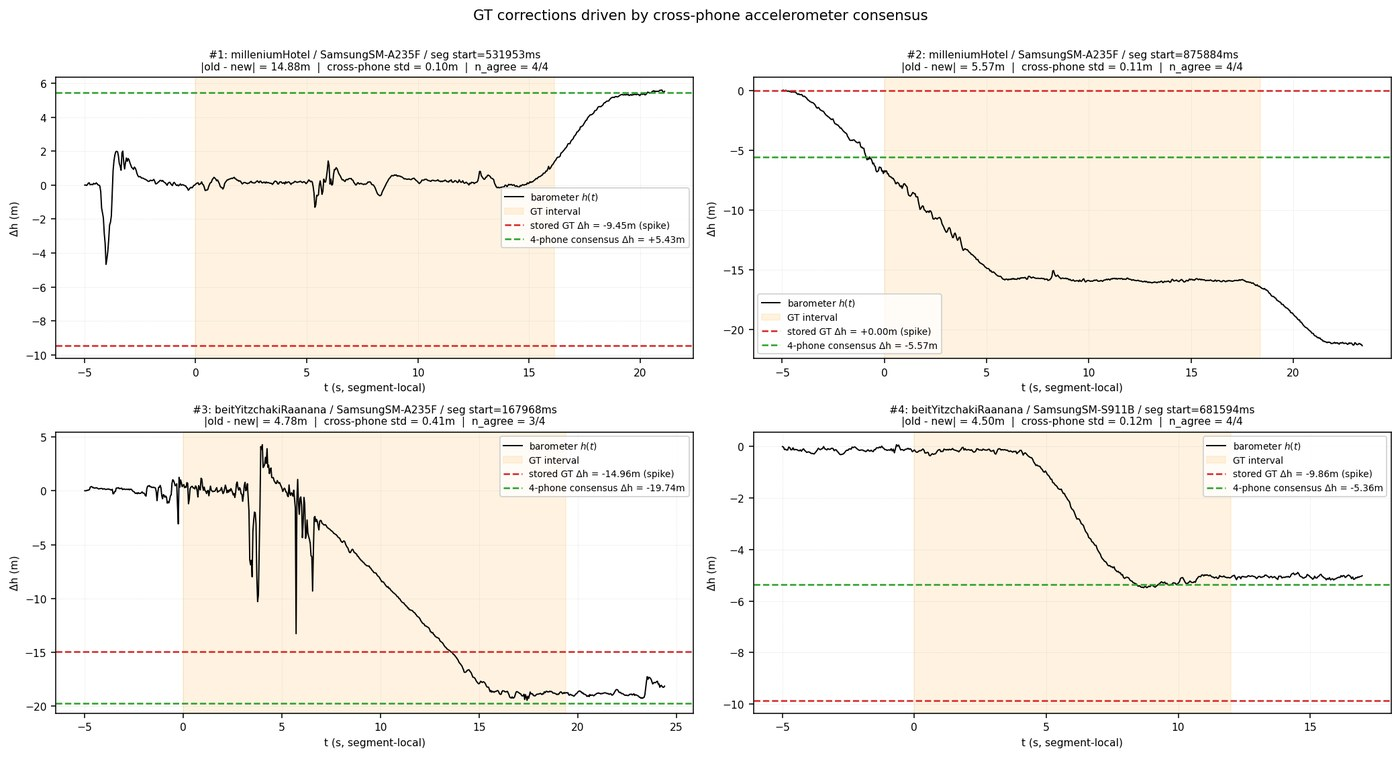
\includegraphics[width=\linewidth, keepaspectratio]{presentation_figs/p072_i0.jpg}
\column{0.48\linewidth}
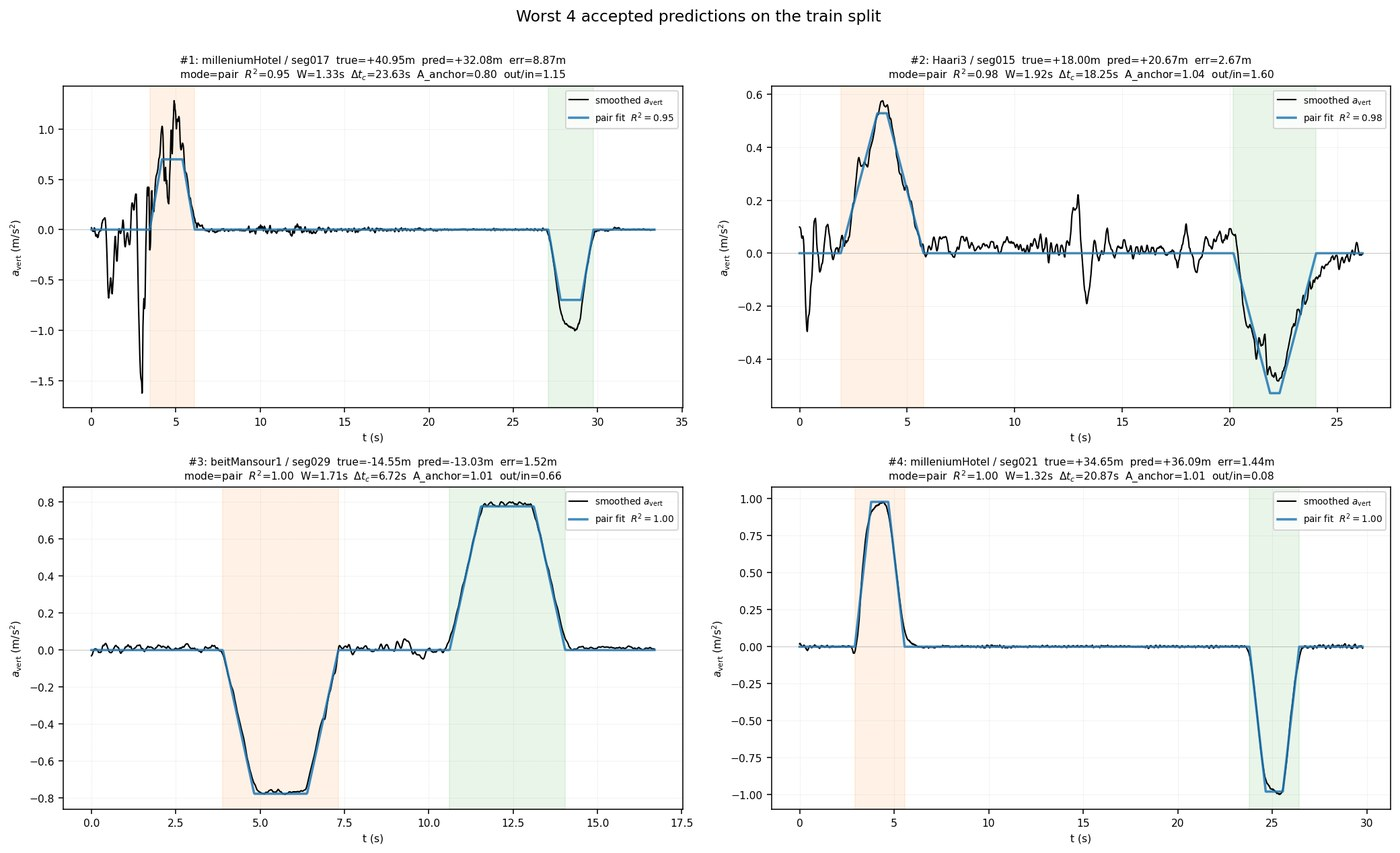
\includegraphics[width=\linewidth, keepaspectratio]{presentation_figs/p073_i0.jpg}
\end{columns}
\par\vspace{0.05cm}
{\footnotesize\itshape\color{pggrey}
Two failure cases. Left: short ride with overlapping lobes. Right: pocket reorient mid-ride.}
\end{frame}


\begin{frame}{Architecture / File Layout}
\textit{Two-stage pipeline; each stage is a Pydantic-configured dispatcher.}\par
\vspace{0.4cm}
\footnotesize
\renewcommand{\arraystretch}{1.5}
\begin{tabular}{@{}p{3.4cm}p{8.4cm}@{}}
\textcolor{pgcopper}{\texttt{src/segmentation/}}  & Stage 1\, --\, \texttt{Segmenter} dispatcher; matched-filter \& pressure-filter algorithms. \\
\textcolor{pgcopper}{\texttt{src/prediction/}}     & Stage 2\, --\, \texttt{Predictor} dispatcher; barometer, ZUPT, trapezoid algorithms. \\
\textcolor{pgcopper}{\texttt{src/utils/}}           & Stage-agnostic helpers\, --\, gravity removal, conformal calibrator, pulse fits. \\
\textcolor{pgcopper}{\texttt{src/data/}}            & Loaders, GT editor, dataset definitions. \\
\textcolor{pgcopper}{\texttt{src/pipelines/}}       & End-to-end Streamlit Boutique Pipeline. \\
\textcolor{pgcopper}{\texttt{docs/latex/}}          & This presentation \& report; LaTeX source + figures. \\
\end{tabular}
\end{frame}


\end{document}
